\section{Experiments}
\label{sec:Experiments}

These experiments were implemented on a set of 12 Modified 3D M-Block modules. The control system which is running the experiments is described in Figure~\ref{fig:electroncsChart}.

\begin{figure}[ht]

	%% Figure of electronics Diagram
\tikzset{box/.style={draw, rectangle, rounded corners, thick, node distance=7em, text width=6em, text centered, minimum height=3.5em}}
\tikzset{container/.style={draw, rectangle, rounded corners, dashed, inner sep=1em}}
\tikzset{line/.style={draw, thick, -latex'}}

\begin{tikzpicture}[auto]
	\node[anchor=south west,inner sep=0, minimum width = \linewidth, minimum height = 8.5cm] (emptyBox) at (0,0) {};
	\begin{scope}[x={(emptyBox.south east)},y={(emptyBox.north west)}]
	\tikzset{>=latex}
		\coordinate (leftCenter) at (0.12, 0.75);
		\coordinate (rightCenter) at (0.6, 0.85);
		\coordinate (routePt) at (0.50, 0.75);
		
		% Main Board
		\node [box] (mainBoard) at (leftCenter) {High Level Control Board (ESP8266)};
		
		% Kyles Boards...
	%	\node [box] at ([shift = ({225:3.5 cm})] mainBoard) (kb) {Motor and Power Board (nRF51422)};
	%	\node [box, right = 1.5cm of kb] (db)  {Actuator Control Board};
		
		% Face Boards
		\node [box] (f0) at (rightCenter) {Face 0 PCB  (IO~Expander)};
		\node [box, below = 0.25cm of f0] (f1) {Face 1 PCB   (IO~Expander)};
		\node [below = 0.75cm of f1] (f2) {...};
		\node [box, below = 0.75cm of f2] (f5) {Face 5 PCB   (IO~Expander)};
		
		%% I2C Connections
		\path [line, <->, orange, ultra thick] (mainBoard) -- (routePt)-- (f0);
		\path [line, <->, orange, ultra thick] (mainBoard) -- (routePt)-- (f1);
		\path [line, <->, orange, ultra thick] (mainBoard) -- (routePt)-- (f5);
		
	%	\path [line, <->, orange, ultra thick] (kb) -- (db);
		
		%% Serial Connections
		
	%	\path [line, <->, blue, ultra thick] (kb) -- (mainBoard);

		%% Inputs
		\node [align = center] (input1) at (0.91, 0.45) {Environmental \\ and \\ Neighbor \\ sensing};
	%	\node [align = left] (input2) at (0.16, 0.96) {wifi commands};

	%	\node [align = left] (input3) at (0.25, 0.24) {Motor \\ Batteries \\ SMA wire};
	%	\node [align = left] (input4) at (0.4, 0.24) {Brake \\ Em coil};
		
%		\draw [dashed,  <->] (kb.south) to [out = 270, in = 180] (input3.west);
%		\draw [dashed,  <->] (input2.south) to [out = 270, in = 235] (mainBoard.west);
%		\draw [dashed,  <->] (input4.east) to [out = 0, in = 325] (db.east);
		
		\draw [dashed,  ->] (input1.north) to [out = 90, in = 0] (f0.east);
		\draw [dashed,  ->] (input1.north) to [out = 90, in = 0] (f1.east);
		\draw [dashed,  ->] (input1.south) to [out = 270, in = 0] (f5.east);
		
		% Dashed Boxes
	%	\node[container, fit = (mainBoard) (kb) (db) (input4) (input3)] (core) {};
	%	\node at (core.south) [below, node distance = 0 and 0] {\textbf{Core}};

		\node[container, fit = (f0) (f5)] (frame) {};
		\node at (frame.south) [below, node distance = 0 and 0] {\textbf{Frame}};

%    	\node [box] (planning) {Planning};
%   	 	\node [box, below of=planning, maroon, inner sep = 0pt] (resources) {Resources};
%   	 	\node [box, below of=resources] (sensors) {Sensors};
%    	\node [box, below of=sensors] (processing) {Processing};
%    	\node [box, below of=sensors] (processing) {Processing};
%    	\node [box, below of=sensors] (processing) {Processing};
%
%    	\coordinate (middle) at ($(resources.west)!0.5!(sensors.west)$);
%    	\node [box, above of=middle, node distance=4 cm] (archive) {Archive};
%    	\node [box, below of=archive, node distance=4 cm] (reporting) {Reporting};
%
%    	\node[container, fit=(resources) (sensors)] (or) {};
%    	\node at (or.north west) [above right,node distance=0 and 0] {OR};
%
%	    \node[container, fit=(archive) (reporting)] (his) {};
%    	\node at (his.north west) [above right,node distance=0 and 0] {HIS};
%
%    	\path [line, line width = 0.5mm, red] (planning) -- (resources);
%    	\path [line] (resources) -- (sensors);
%    	\path [line] (sensors) -- (processing);
%
%    	\path [line] (archive) |- (planning);
%    	\path [line] (archive) |- (processing);
%    	\path [line] (processing)--($(processing.south)-(0,0.5)$) -| (reporting);
%
%    	\draw [line] ($(processing.south)-(0,0.5)$) -- ++(4,0) node(lowerright){} |- (planning.east);
%    	\draw [line] (lowerright |- or.east) -- (or.east -| resources.south east);
%
%    	\draw[line] (archive.170)--(reporting.10);
%    	\draw[line] (reporting.350)--(archive.190);
    \end{scope}
\end{tikzpicture}


%
%
%	\begin{tikzpicture}
%	\node[anchor=south west,inner sep=0] (image) at (0,0) {\includegraphics[width=0.9\textwidth]{some_image.jpg}};
%	\begin{scope}[x={(image.south east)},y={(image.north west)}]
%
%	\end{scope}
%	\end{tikzpicture}
%\end{document}
	
\caption{This figure illustrates the various avenues of information exchange between the different elements of the experimental setup. The \emph{orange} arrows represent bi-directional WIFI messages sent between the immobile \emph{Server Module} and the active modules, with the dashed line showing a potentially faulty connection. The \emph{blue} arrows show the simple light-based messages which active modules are able to send to neighbors that they are directly connected to. The \emph{purple} arrows represent the reading of \tagNamePlural~ between an active module and a valid and adjacently connected \tagName. Note that \tagNamePlural can be read from both passive modules, and from passive or even unresponsive modules.}
	
	\label{fig:electroncsChart}
\end{figure}



%%%%%%%%%%%%%%%%%%%%%%%%%%%%%%%%%%%%%%%%%%%%%%%%%%%%%%%%%%%%%%%%%%%%%%%%%%%%%%%%%%%%%%%%%%%%%%%%%%%%%%%%%%%%%%%%%%%%%%%%%%%%%%%%%%%%%%%%%%%%%%%
%%%%%%%%%%%%%%%%%%%%%%%%%%%%%%%%%%%%%%%%%%%%%%%%%%%%%%%%%%%%%%%%%%%%%%%%%%%%%%%%%%%%%%%%%%%%%%%%%%%%%%%%%%%%%%%%%%%%%%%%%%%%%%%%%%%%%%%%%%%%%%%
\subsection{Arrow Following experiments}
\label{sec:mblocksExperimentsArrow}
%%%%%%%%%%%%%%%%%%%%%%%%%%%%%%%%%%%%%%%%%%%%%%%%%%%%%%%%%%%%%%%%%%%%%%%%%%%%%%%%%%%%%%%%%%%%%%%%%%%%%%%%%%%%%%%%%%%%%%%%%%%%%%%%%%%%%%%%%%%%%%%
%%%%%%%%%%%%%%%%%%%%%%%%%%%%%%%%%%%%%%%%%%%%%%%%%%%%%%%%%%%%%%%%%%%%%%%%%%%%%%%%%%%%%%%%%%%%%%%%%%%%%%%%%%%%%%%%%%%%%%%%%%%%%%%%%%%%%%%%%%%%%%%
This experiment tested the ability of the Modules to identify and follow the "arrows" embedded in in a set of passive modules. The experiment consisted of a single module 
implementing the algorithm in... 

\begin{table}[h]
	\caption{Experimental results Table}
	
	\begin{tabular}{ p{2.2cm}  p{1.2cm}  p{1.2cm} p{1.2cm}}
		\hline
							& runs 	& Success & moves \\
		\hline
		Line Formation		&  1 		& 5/8 		& 6\\
		Light Aggregation 	&  1 		& 4/12 		& 20\\		
		Path Following		&  1 		& 1/1 		& 2 \\
		Extended Path		&	0		&0			& 0\\

	\end{tabular}
	
	\label{tab:info}
\end{table}

\begin{figure}[h]  
	\centering
	\begin{subfigure}[b]{0.32\linewidth}
		\begin{tikzpicture}[]	
		\node[opacity = 0.95] at (0,0) {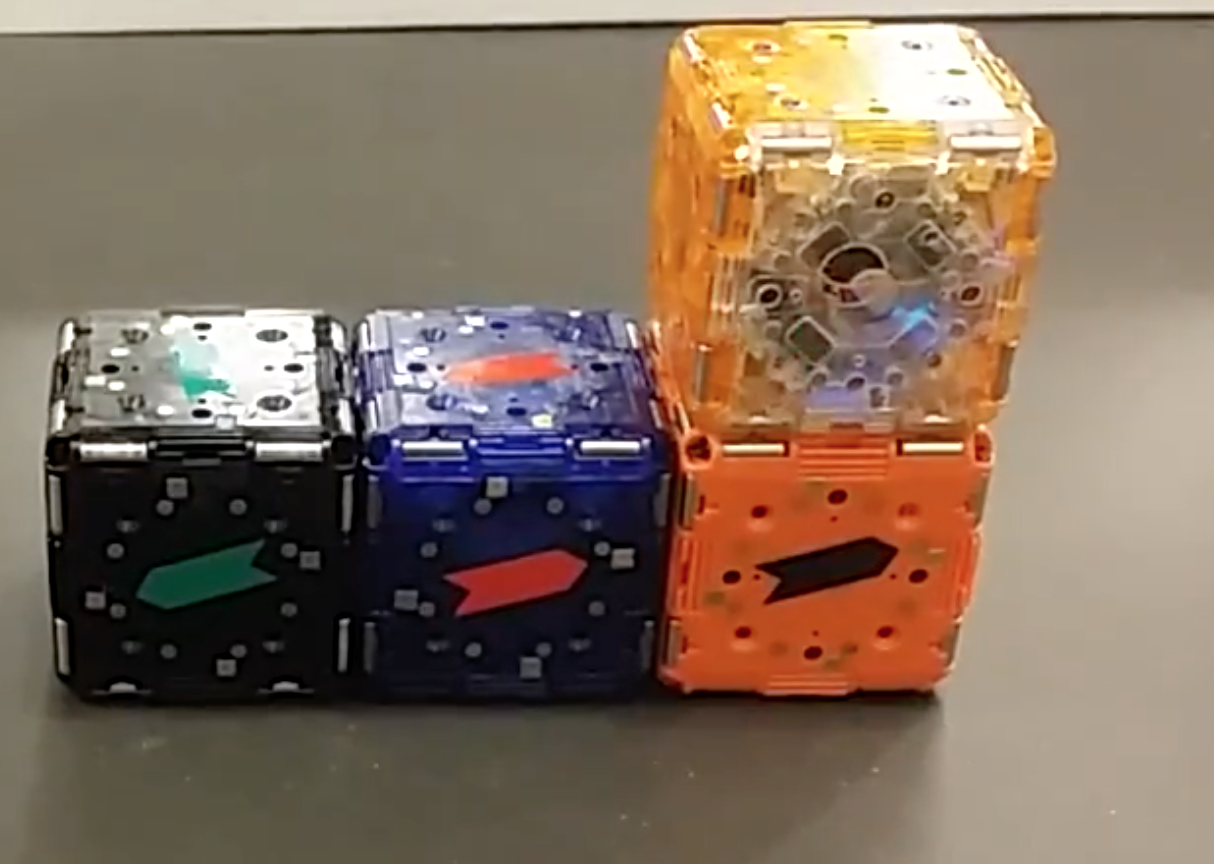
\includegraphics[width=0.95\linewidth]{figures/arrows2.png}};
		\node[opacity = 0.5, fill = white, rounded corners] at (-0.5,-0.75) {t = 0 s};
		\end{tikzpicture}
	\end{subfigure}
	\begin{subfigure}[b]{0.32\linewidth}
		\begin{tikzpicture}[]	
		\node[opacity = 0.95] at (0,0) {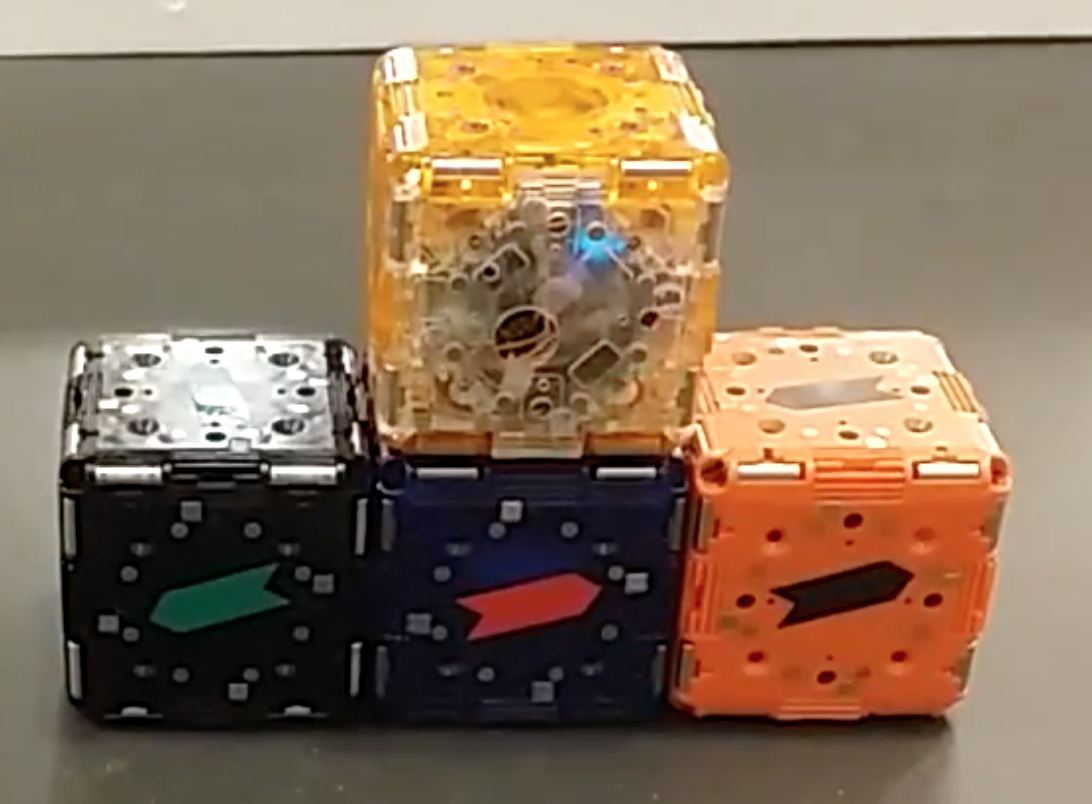
\includegraphics[width=0.95\linewidth]{figures/arrows3.png}};
		\node[opacity = 0.5, fill = white, rounded corners] at (-0.5,-0.75) {t = 50 s};
		\end{tikzpicture}
	\end{subfigure}
	\begin{subfigure}[b]{0.32\linewidth}
		\begin{tikzpicture}[]	
		\node[opacity = 0.95] at (0,0) {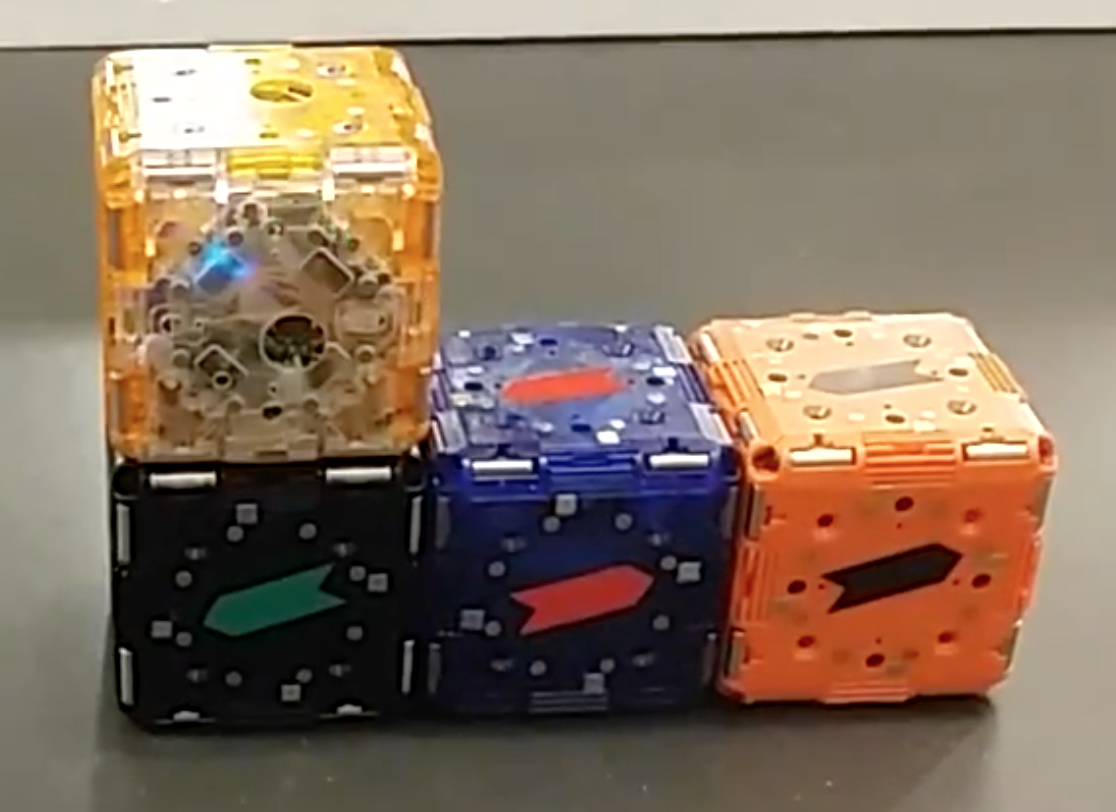
\includegraphics[width=0.95\linewidth]{figures/arrows4.png}};
		\node[opacity = 0.5, fill = white, rounded corners] at (-0.5,-0.75) {t = 120 s};
		\end{tikzpicture}
	\end{subfigure}
	
	\caption{This experiment the cube following a very simple embedded arrow path.}
	
	\label{fig:arrowExperiment}
\end{figure}

%%%%%%%%%%%%%%%%%%%%%%%%%%%%%%%%%%%%%%%%%%%%%%%%%%%%%%%%%%%%%%%%%%%%%%%%%%%%%%%%%%%%%%%%%%%%%%%%%%%%%%%%%%%%%%%%%%%%%%%%%%%%%%%%%%%%%%%%%%%%%%%
%%%%%%%%%%%%%%%%%%%%%%%%%%%%%%%%%%%%%%%%%%%%%%%%%%%%%%%%%%%%%%%%%%%%%%%%%%%%%%%%%%%%%%%%%%%%%%%%%%%%%%%%%%%%%%%%%%%%%%%%%%%%%%%%%%%%%%%%%%%%%%%
\subsection{Line formation experiments}
\label{sec:mblocksExperimentsLine}
%%%%%%%%%%%%%%%%%%%%%%%%%%%%%%%%%%%%%%%%%%%%%%%%%%%%%%%%%%%%%%%%%%%%%%%%%%%%%%%%%%%%%%%%%%%%%%%%%%%%%%%%%%%%%%%%%%%%%%%%%%%%%%%%%%%%%%%%%%%%%%%
%%%%%%%%%%%%%%%%%%%%%%%%%%%%%%%%%%%%%%%%%%%%%%%%%%%%%%%%%%%%%%%%%%%%%%%%%%%%%%%%%%%%%%%%%%%%%%%%%%%%%%%%%%%%%%%%%%%%%%%%%%%%%%%%%%%%%%%%%%%%%%%

These experiments involved several attempts to convert arbitrary generated 3D structures with a few constraints (no holes, and no modules connected by three or more connection faces) into a single horizontal line involving between 8 and 12 modules.

\begin{figure}[h]  
	\centering
	\begin{subfigure}[b]{0.32\linewidth}
		\begin{tikzpicture}[]	
			\node[opacity = 0.95] at (0,0) {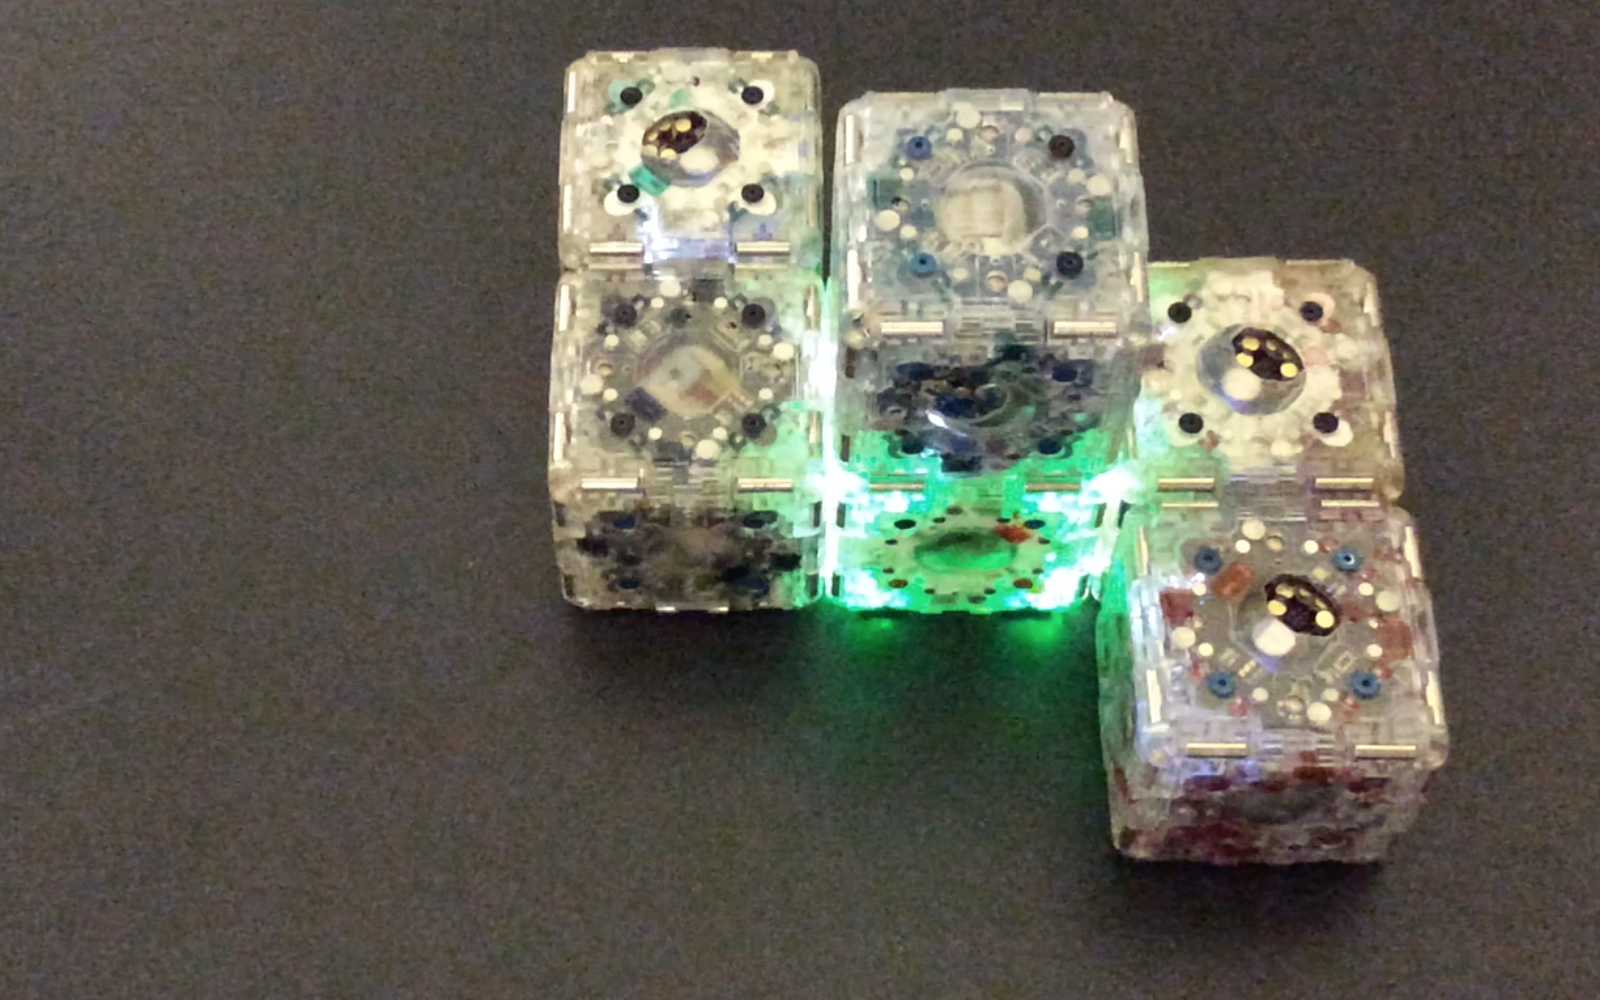
\includegraphics[width=0.95\linewidth]{figures/ActualLine_1.png}};
			\node[opacity = 0.5, fill = white, rounded corners] at (-0.5,-0.5) {t = 0 s};
		\end{tikzpicture} 
	\end{subfigure}
	\begin{subfigure}[b]{0.32\linewidth}
			\begin{tikzpicture}[]	
		\node[opacity = 0.95] at (0,0) {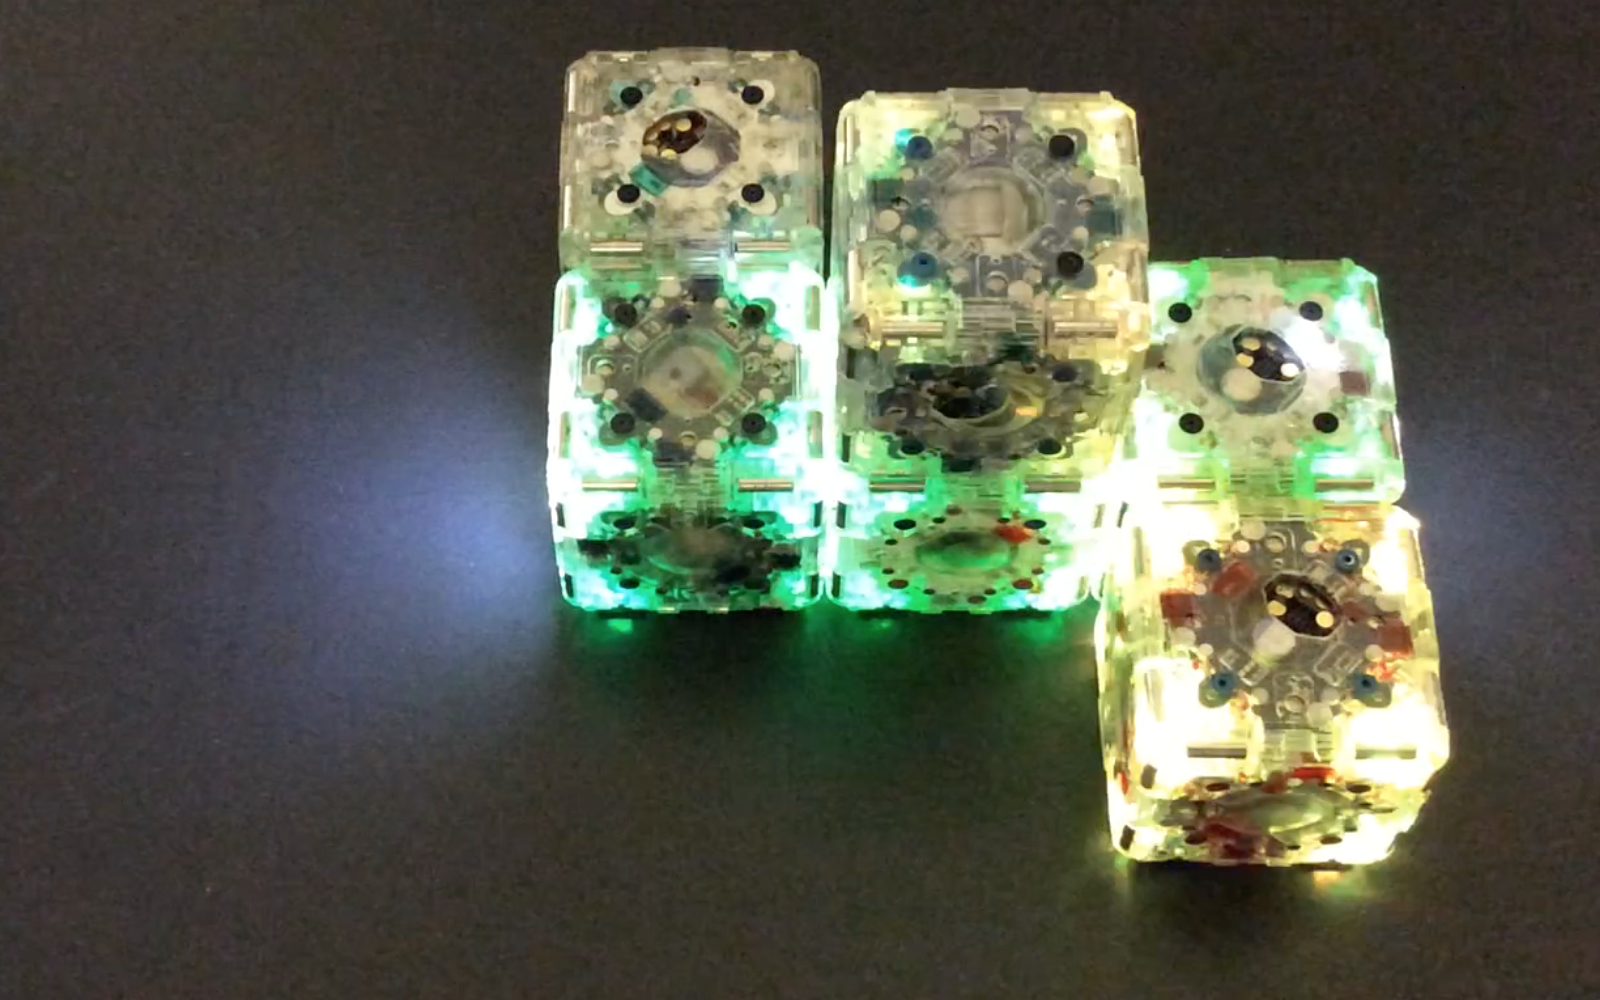
\includegraphics[width=0.95\linewidth]{figures/ActualLine_2.png}};
		\node[opacity = 0.5, fill = white, rounded corners] at (-0.5,-0.5) {t = 30 s};
		\end{tikzpicture}
	\end{subfigure}
	\begin{subfigure}[b]{0.32\linewidth}
			\begin{tikzpicture}[]	
		\node[opacity = 0.95] at (0,0) {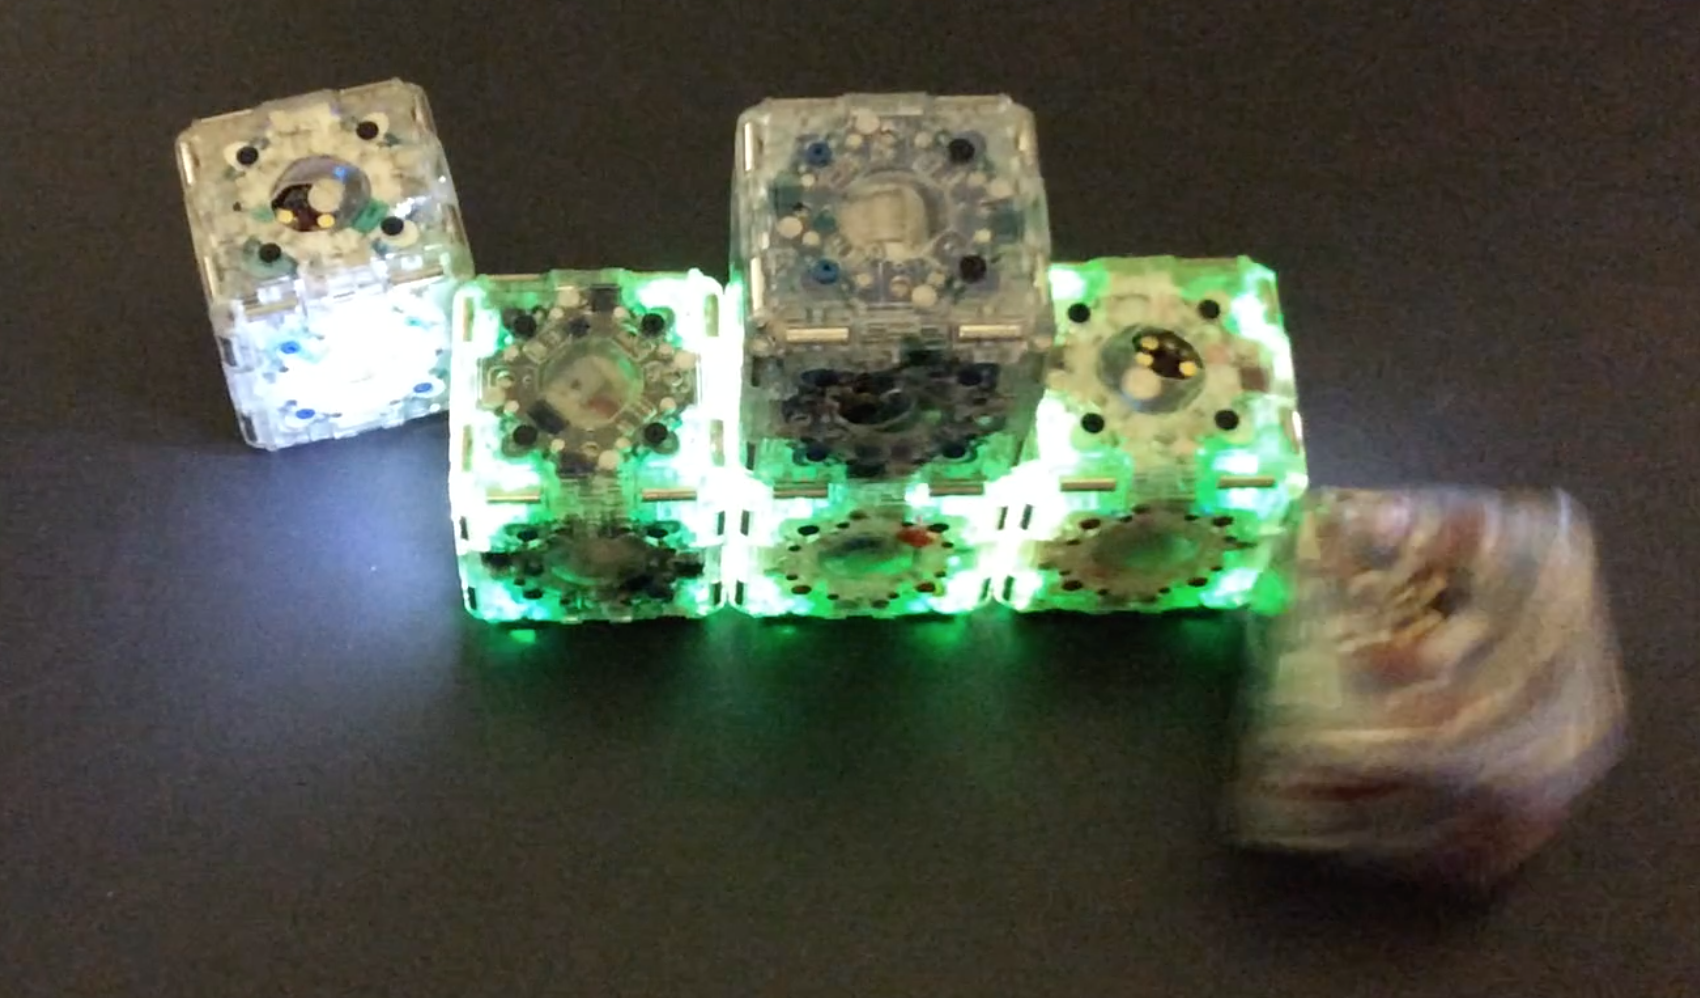
\includegraphics[width=0.95\linewidth]{figures/ActualLine_3.png}};
		\node[opacity = 0.5, fill = white, rounded corners] at (-0.5,-0.5) {t = 60 s};
		\end{tikzpicture}
	\end{subfigure}

	\begin{subfigure}[b]{0.32\linewidth}
			\begin{tikzpicture}[]	
		\node[opacity = 0.95] at (0,0) {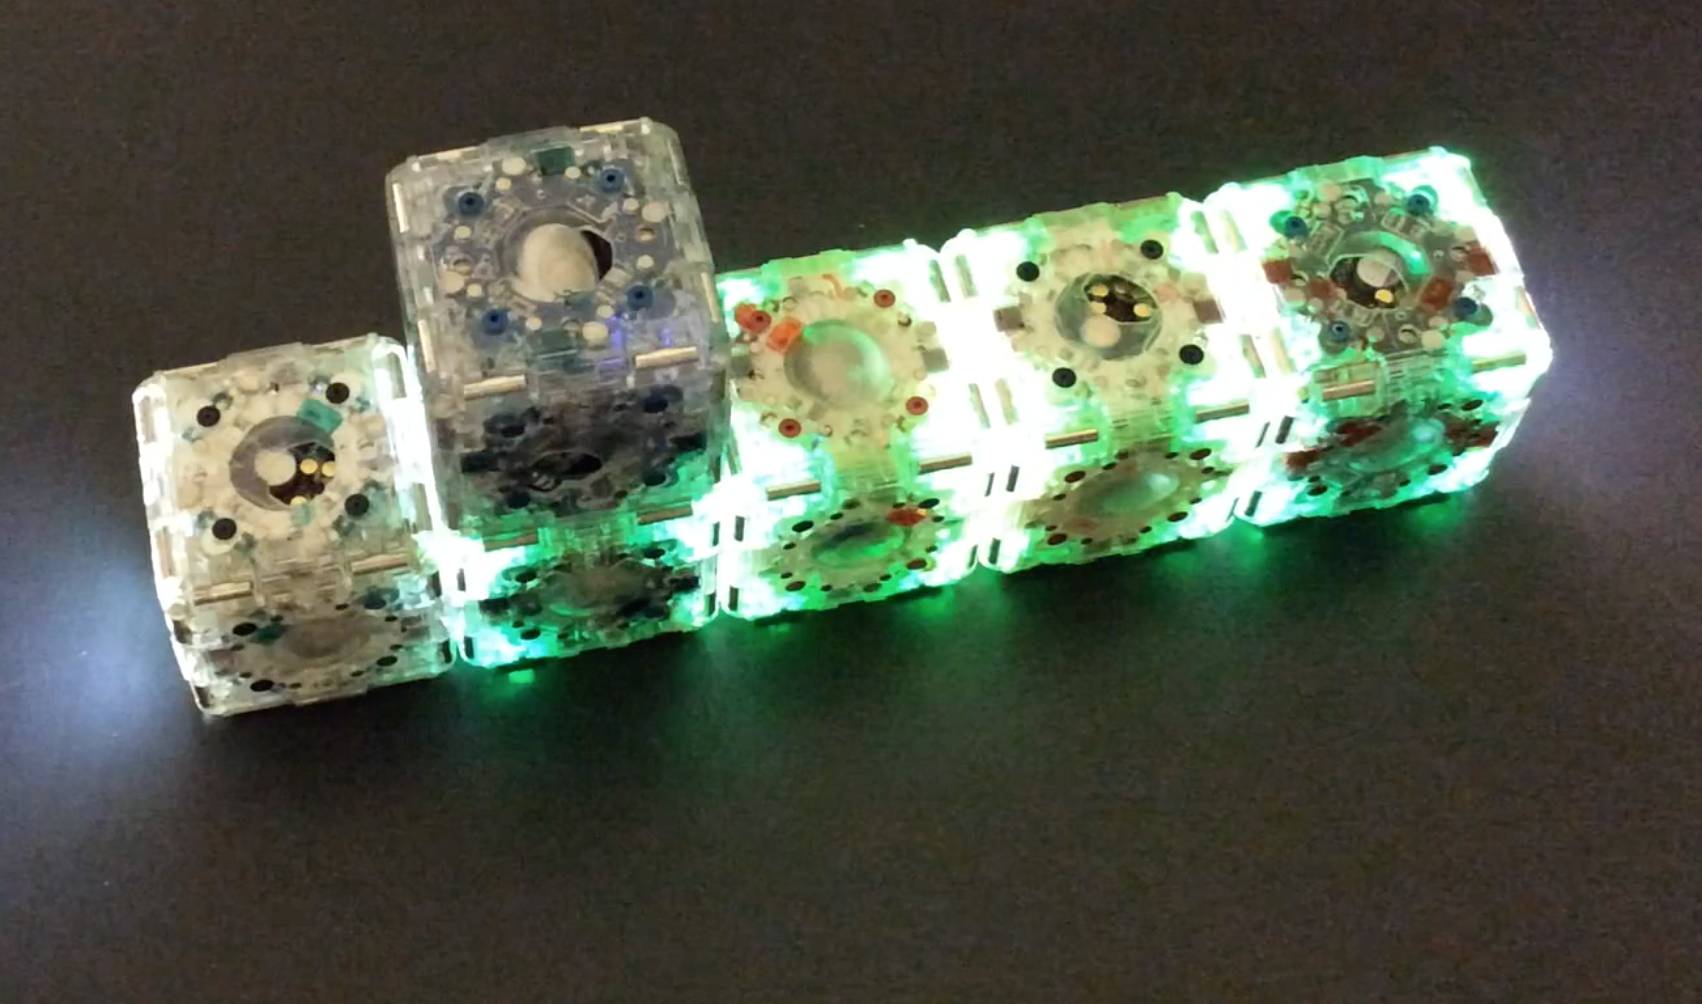
\includegraphics[width=0.95\linewidth]{figures/ActualLine_4.png}};
		\node[opacity = 0.5, fill = white, rounded corners] at (-0.5,-0.5) {t = 120 s};
		\end{tikzpicture}
	\end{subfigure}
	\begin{subfigure}[b]{0.32\linewidth}
			\begin{tikzpicture}[]	
		\node[opacity = 0.95] at (0,0) {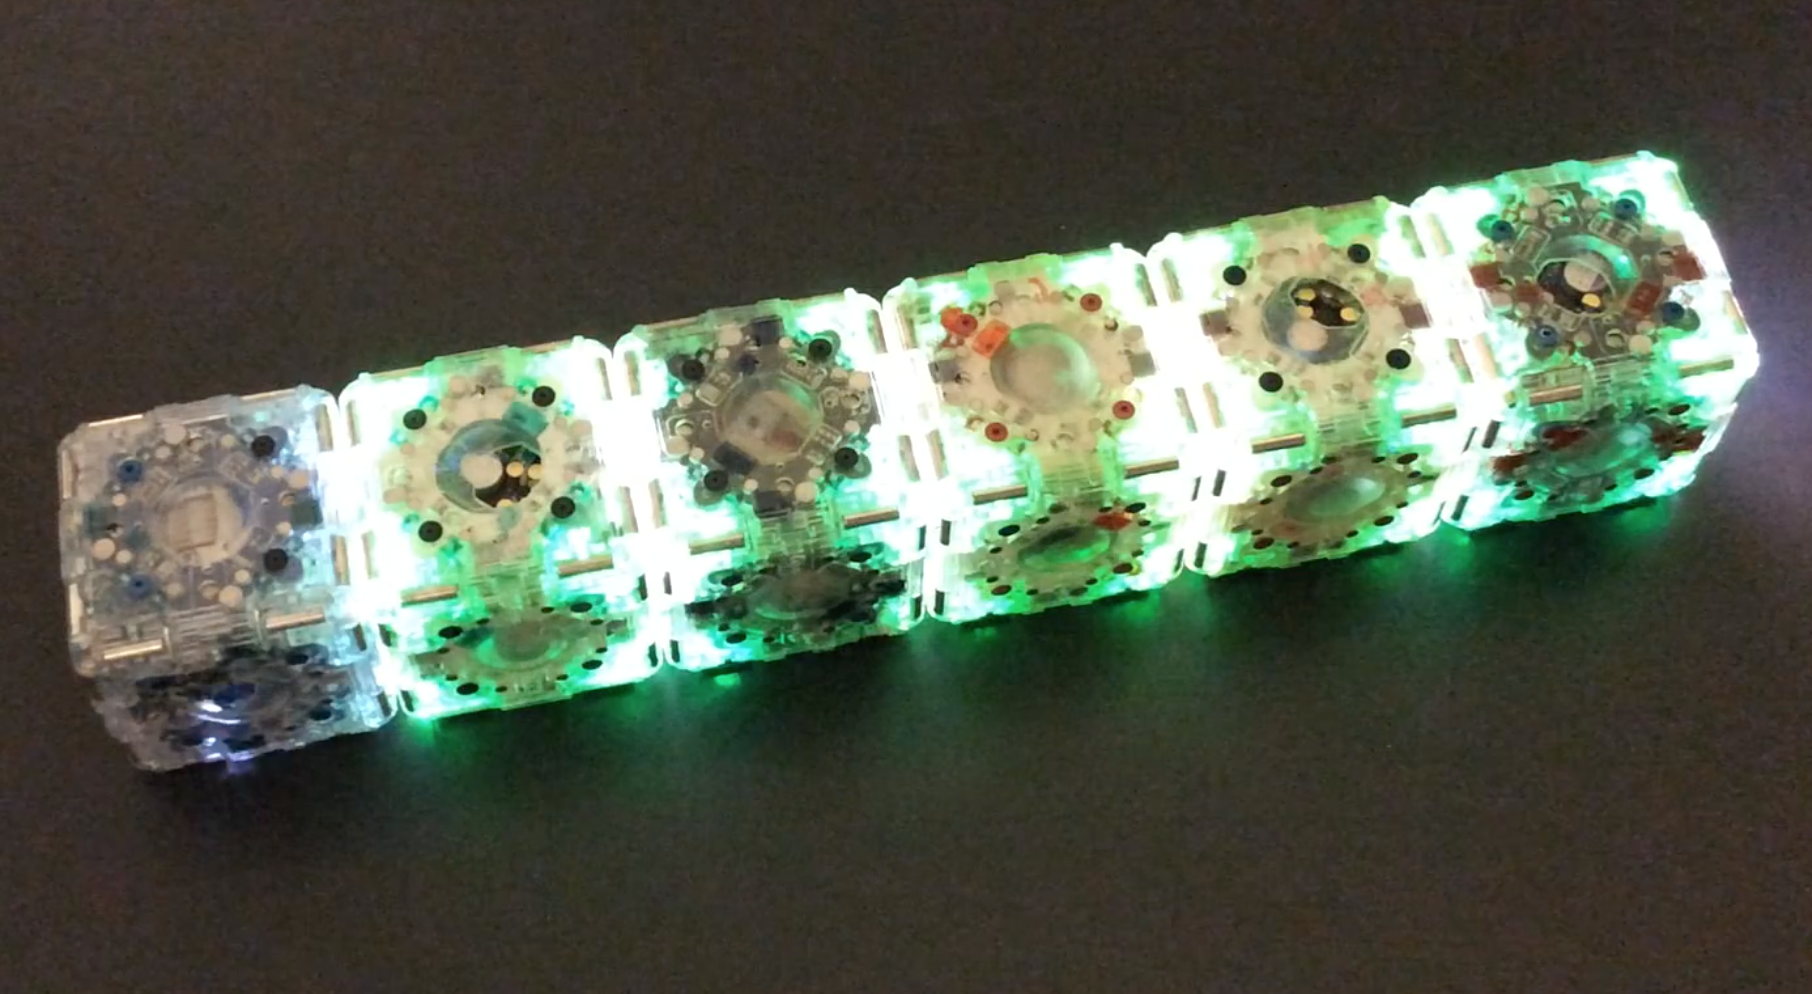
\includegraphics[width=0.95\linewidth]{figures/ActualLine_5.png}};
		\node[opacity = 0.5, fill = white, rounded corners] at (-0.5,-0.5) {t = 230 s};
		\end{tikzpicture}
	\end{subfigure}
	\begin{subfigure}[b]{0.32\linewidth}
			\begin{tikzpicture}[]	
		\node[opacity = 0.95] at (0,0) {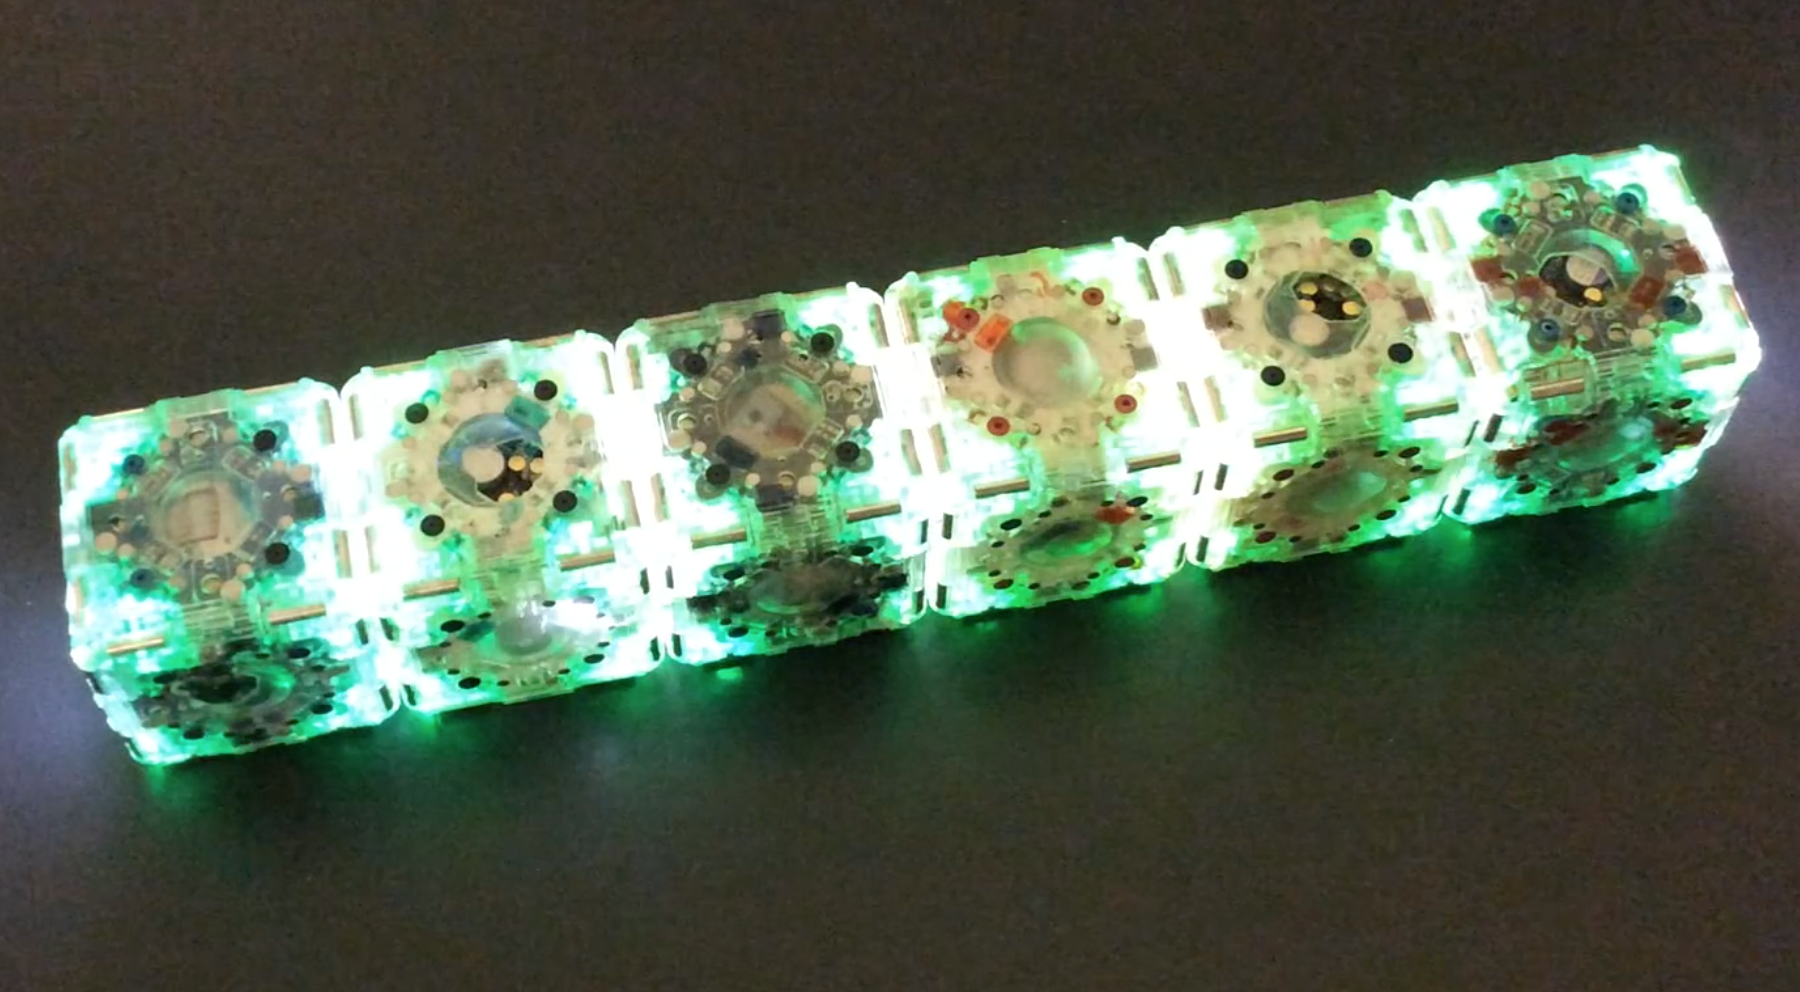
\includegraphics[width=0.95\linewidth]{figures/ActualLine_6.png}};
		\node[opacity = 0.5, fill = white, rounded corners] at (-0.5,-0.5) {t = 300 s};
		\end{tikzpicture}
	\end{subfigure}
	
	\caption{This experiment shows a random 3D configuration of M-Blocks reconfiguring into a line.}
	
	\label{fig:lineExperiment}
\end{figure}

%%%%%%%%%%%%%%%%%%%%%%%%%%%%%%%%%%%%%%%%%%%%%%%%%%%%%%%%%%%%%%%%%%%%%%%%%%%%%%%%%%%%%%%%%%%%%%%%%%%%%%%%%%%%%%%%%%%%%%%%%%%%%%%%%%%%%%%%%%%%%%%
%%%%%%%%%%%%%%%%%%%%%%%%%%%%%%%%%%%%%%%%%%%%%%%%%%%%%%%%%%%%%%%%%%%%%%%%%%%%%%%%%%%%%%%%%%%%%%%%%%%%%%%%%%%%%%%%%%%%%%%%%%%%%%%%%%%%%
\subsection{Light guided aggregation experiments}
\label{sec:mblocksExperimentsLight}
%%%%%%%%%%%%%%%%%%%%%%%%%%%%%%%%%%%%%%%%%%%%%%%%%%%%%%%%%%%%%%%%%%%%%%%%%%%%%%%%%%%%%%%%%%%%%%%%%%%%%%%%%%%%%%%%%%%%%%%%%%%%%%%%%%%%%%%%%%%%%%%
%%%%%%%%%%%%%%%%%%%%%%%%%%%%%%%%%%%%%%%%%%%%%%%%%%%%%%%%%%%%%%%%%%%%%%%%%%%%%%%%%%%%%%%%%%%%%%%%%%%%%%%%%%%%%%%%%%%%%%%%%%%%%%%%%%%%%%%%%%%%%%%


These experiments essentially attempt to implement the photo-taxis Braitenberg behavior for a group of M-Blocks modules. There is a single light source, and a special target module, which when modules aggregate to it, the modules share its location through wireless and light signals for additional modules to connect to it - essentially forming a single "crystal" of aggregated modules. In these experiment modules are gradually released into a confined (0.5m x 0.5 m) bounded foam-padded location, and move until they either run out of battery or connect to the designated aggregate.

%\newcommand{\figureWidth}{0.32\linewidth}
\begin{figure}[h]  
	\centering
	\begin{subfigure}[b]{0.32\linewidth}
		
		\begin{tikzpicture}[]	
			\node[opacity = 0.95] at (0,0) {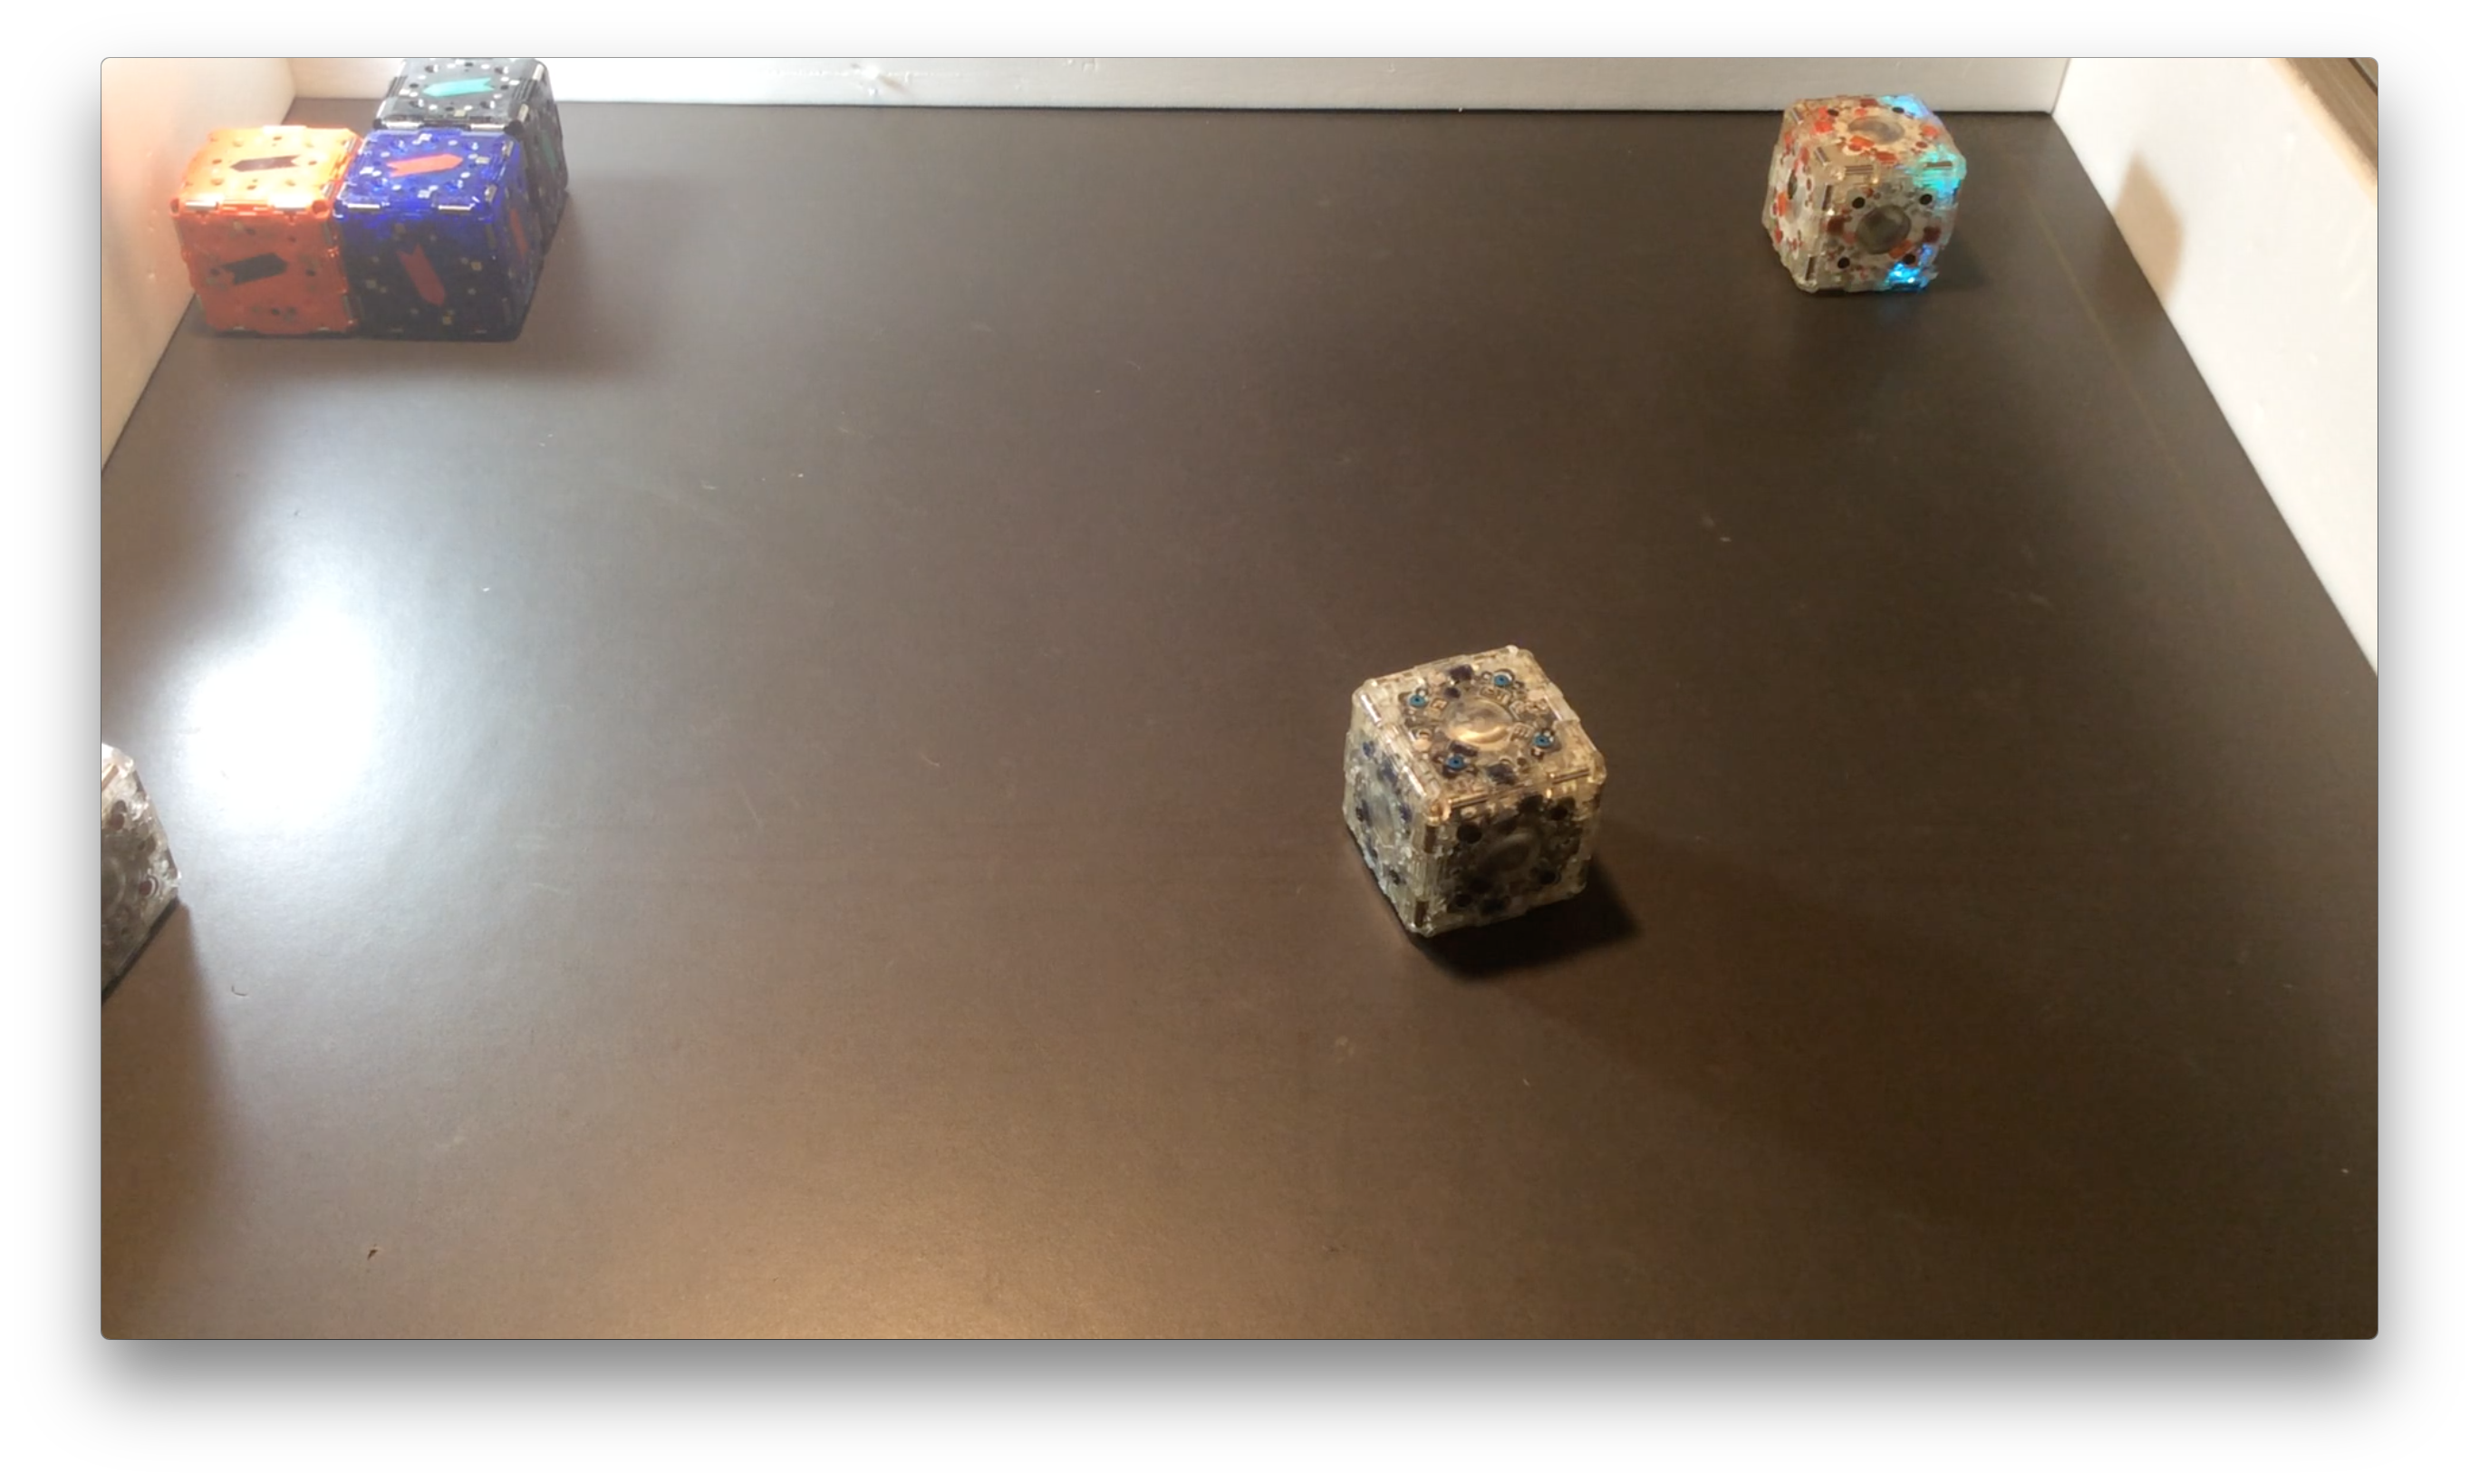
\includegraphics[width = \linewidth]{figures/1-000.png}};
			\node[opacity = 0.5, fill = white, rounded corners] at (-0.5,-0.5) {t = 000 s};
		\end{tikzpicture}
		
	\end{subfigure}
	\begin{subfigure}[b]{0.32\linewidth}
		
		\begin{tikzpicture}[]	
		\node[opacity = 0.95] at (0,0) {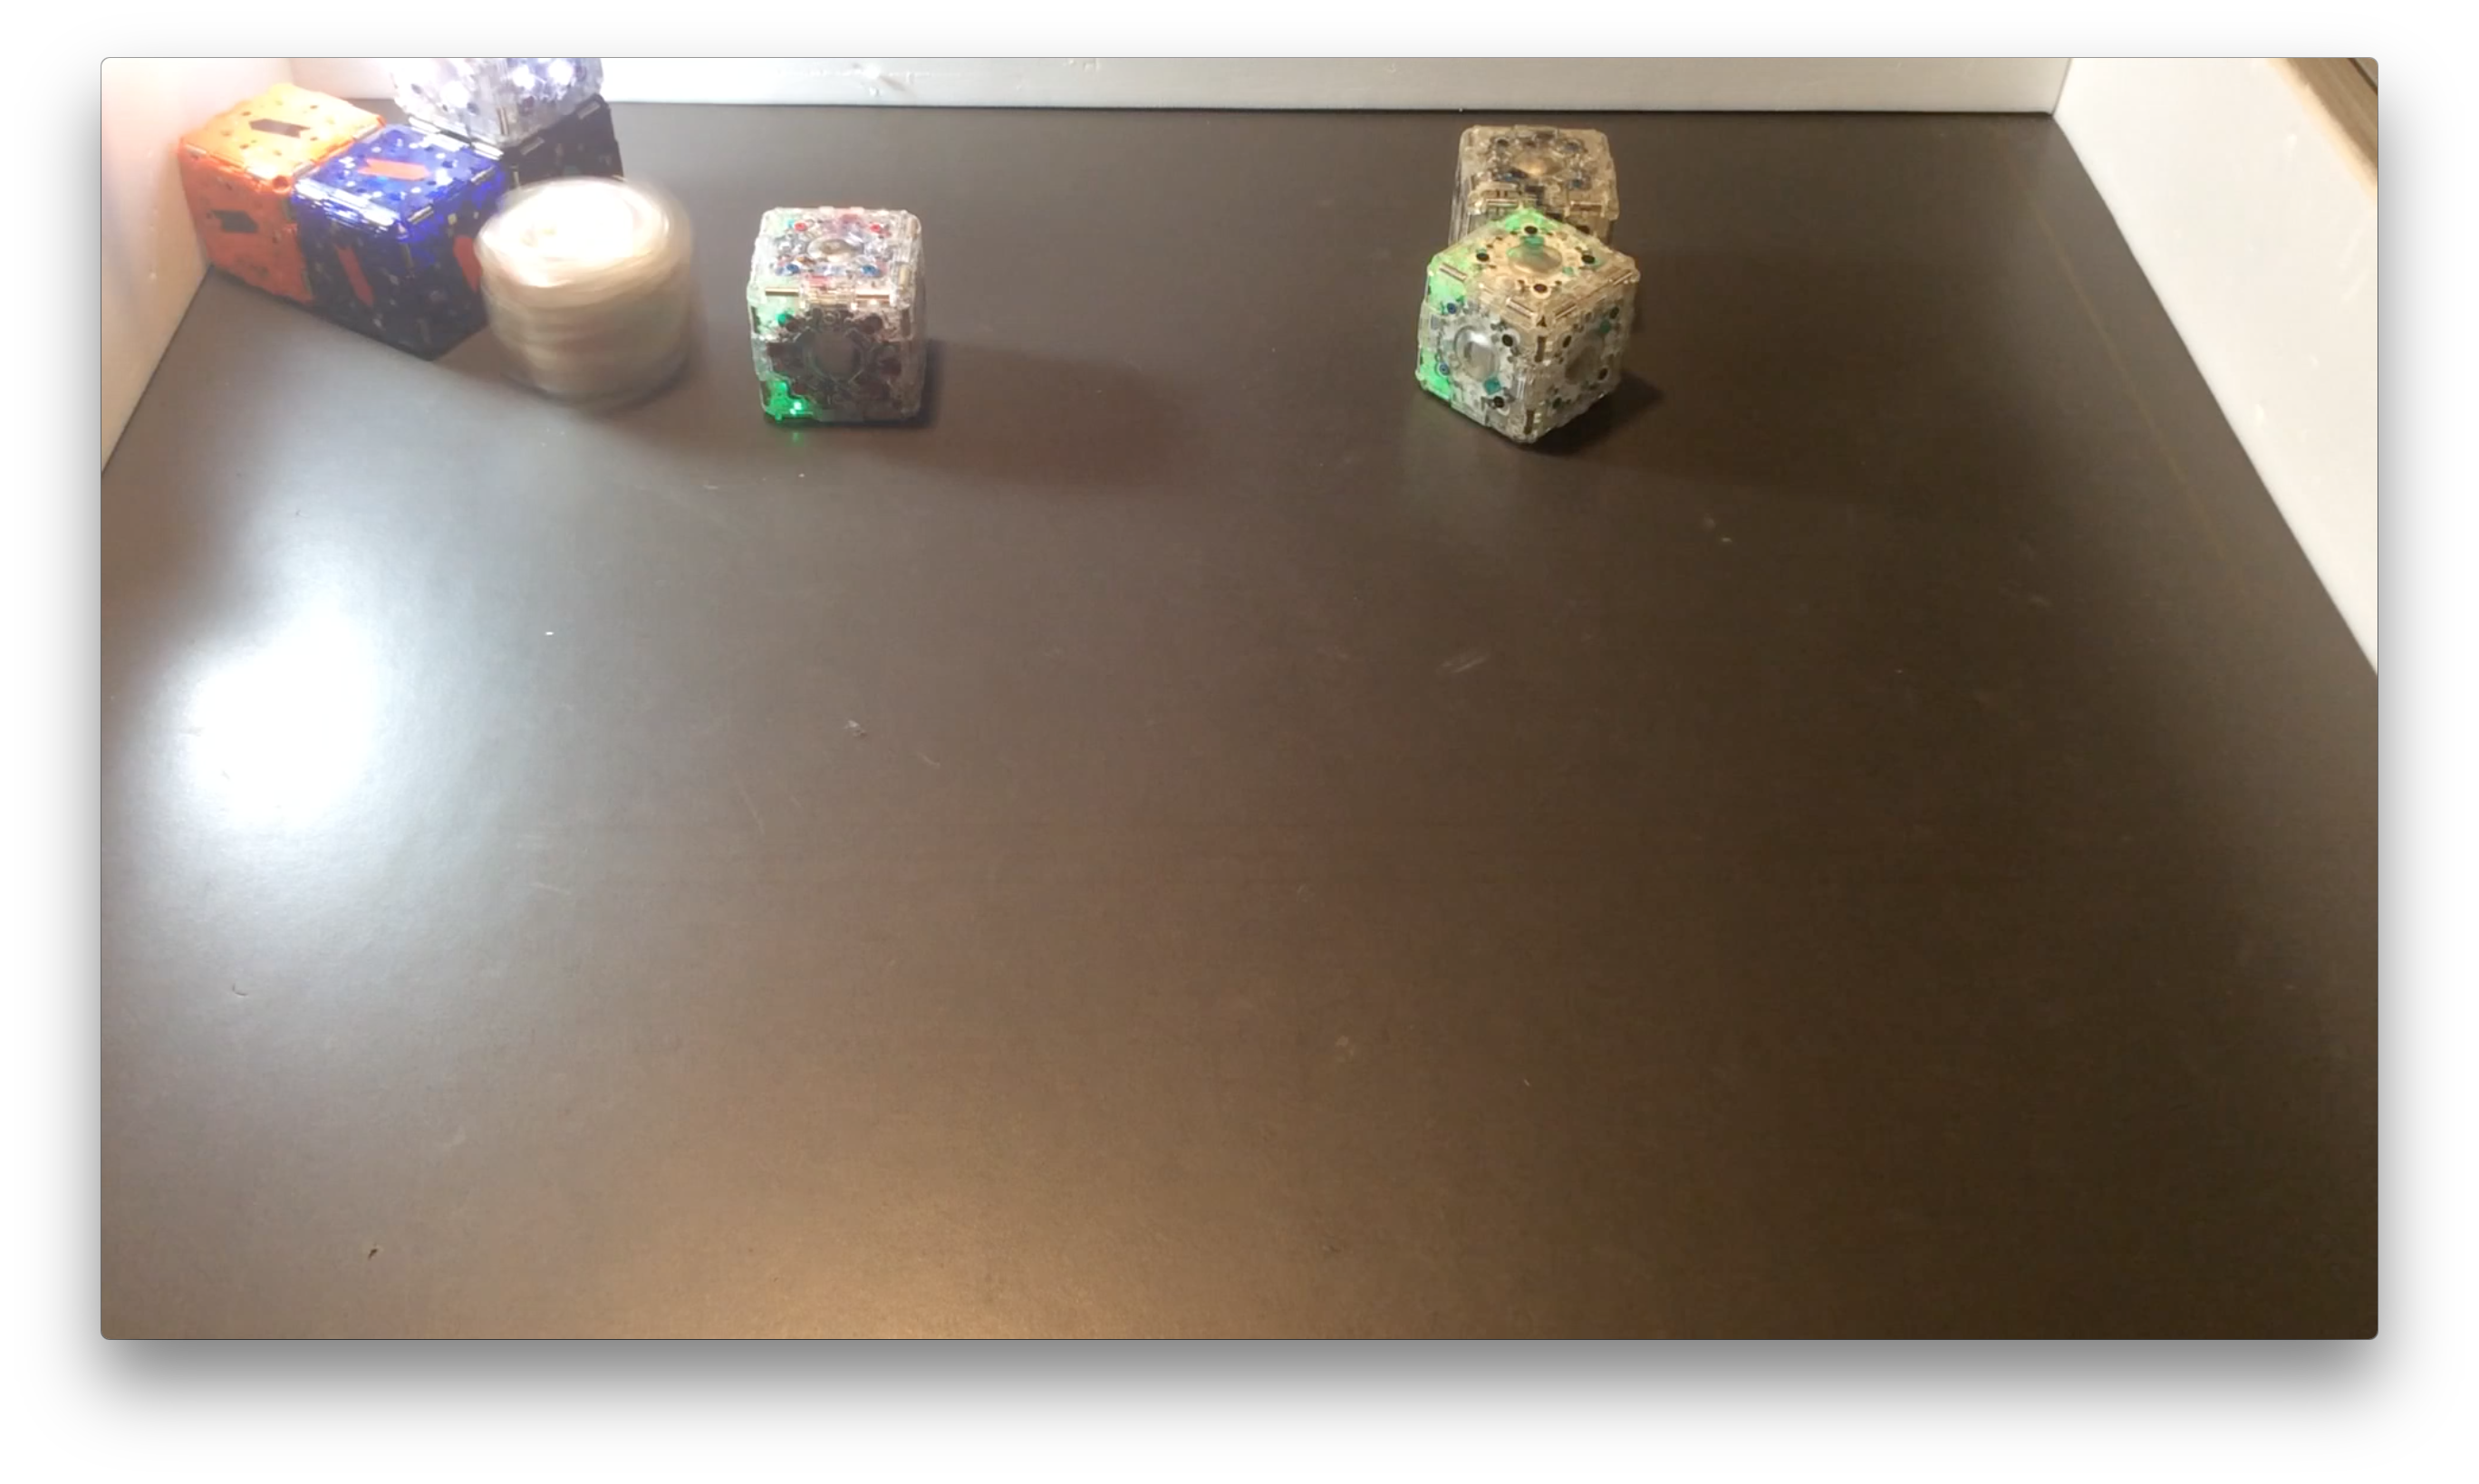
\includegraphics[width = \linewidth]{figures/2-120.png}};
		\node[opacity = 0.5, fill = white, rounded corners] at (-0.5,-0.5) {t = 120 s};
		\end{tikzpicture}
		
	\end{subfigure}
	\begin{subfigure}[b]{0.32\linewidth}

		\begin{tikzpicture}[]	
		\node[opacity = 0.95] at (0,0) {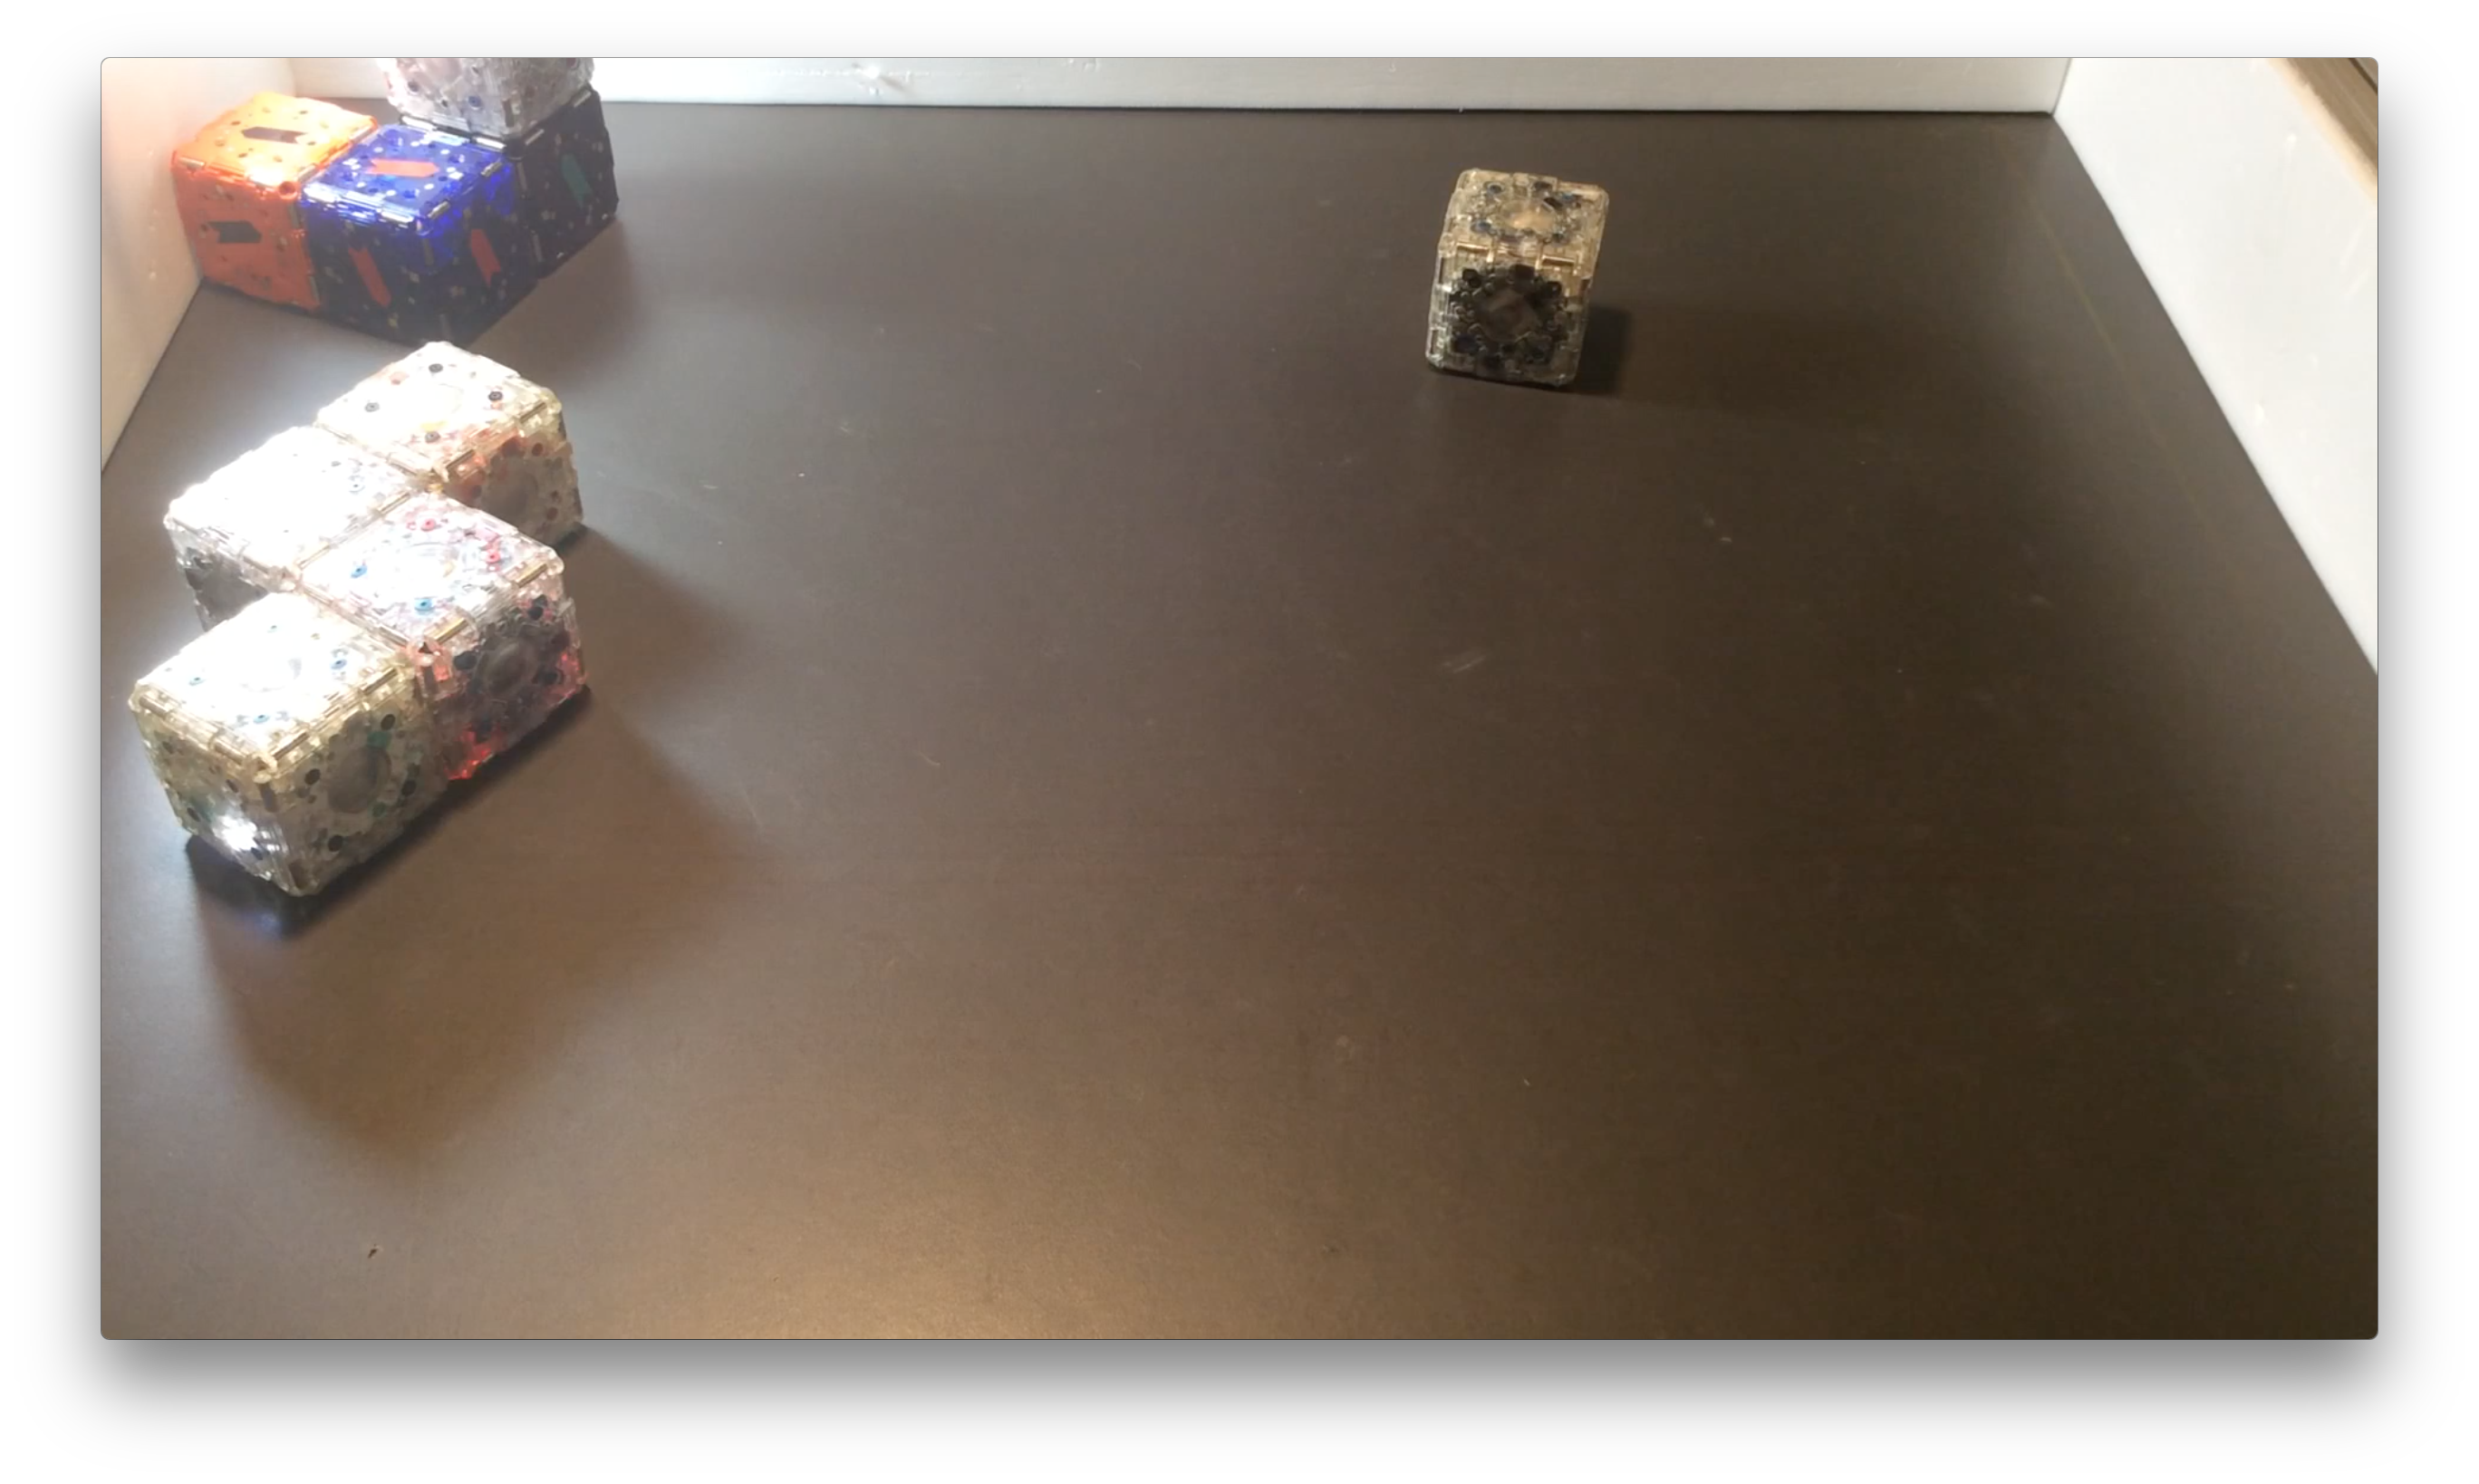
\includegraphics[width = \linewidth]{figures/3-220.png}};
		\node[opacity = 0.5, fill = white, rounded corners] at (-0.5,-0.5) {t = 220 s};
		\end{tikzpicture}
		
	\end{subfigure}

	\begin{subfigure}[b]{0.32\linewidth}
		\begin{tikzpicture}[]	
		\node[opacity = 0.95] at (0,0) {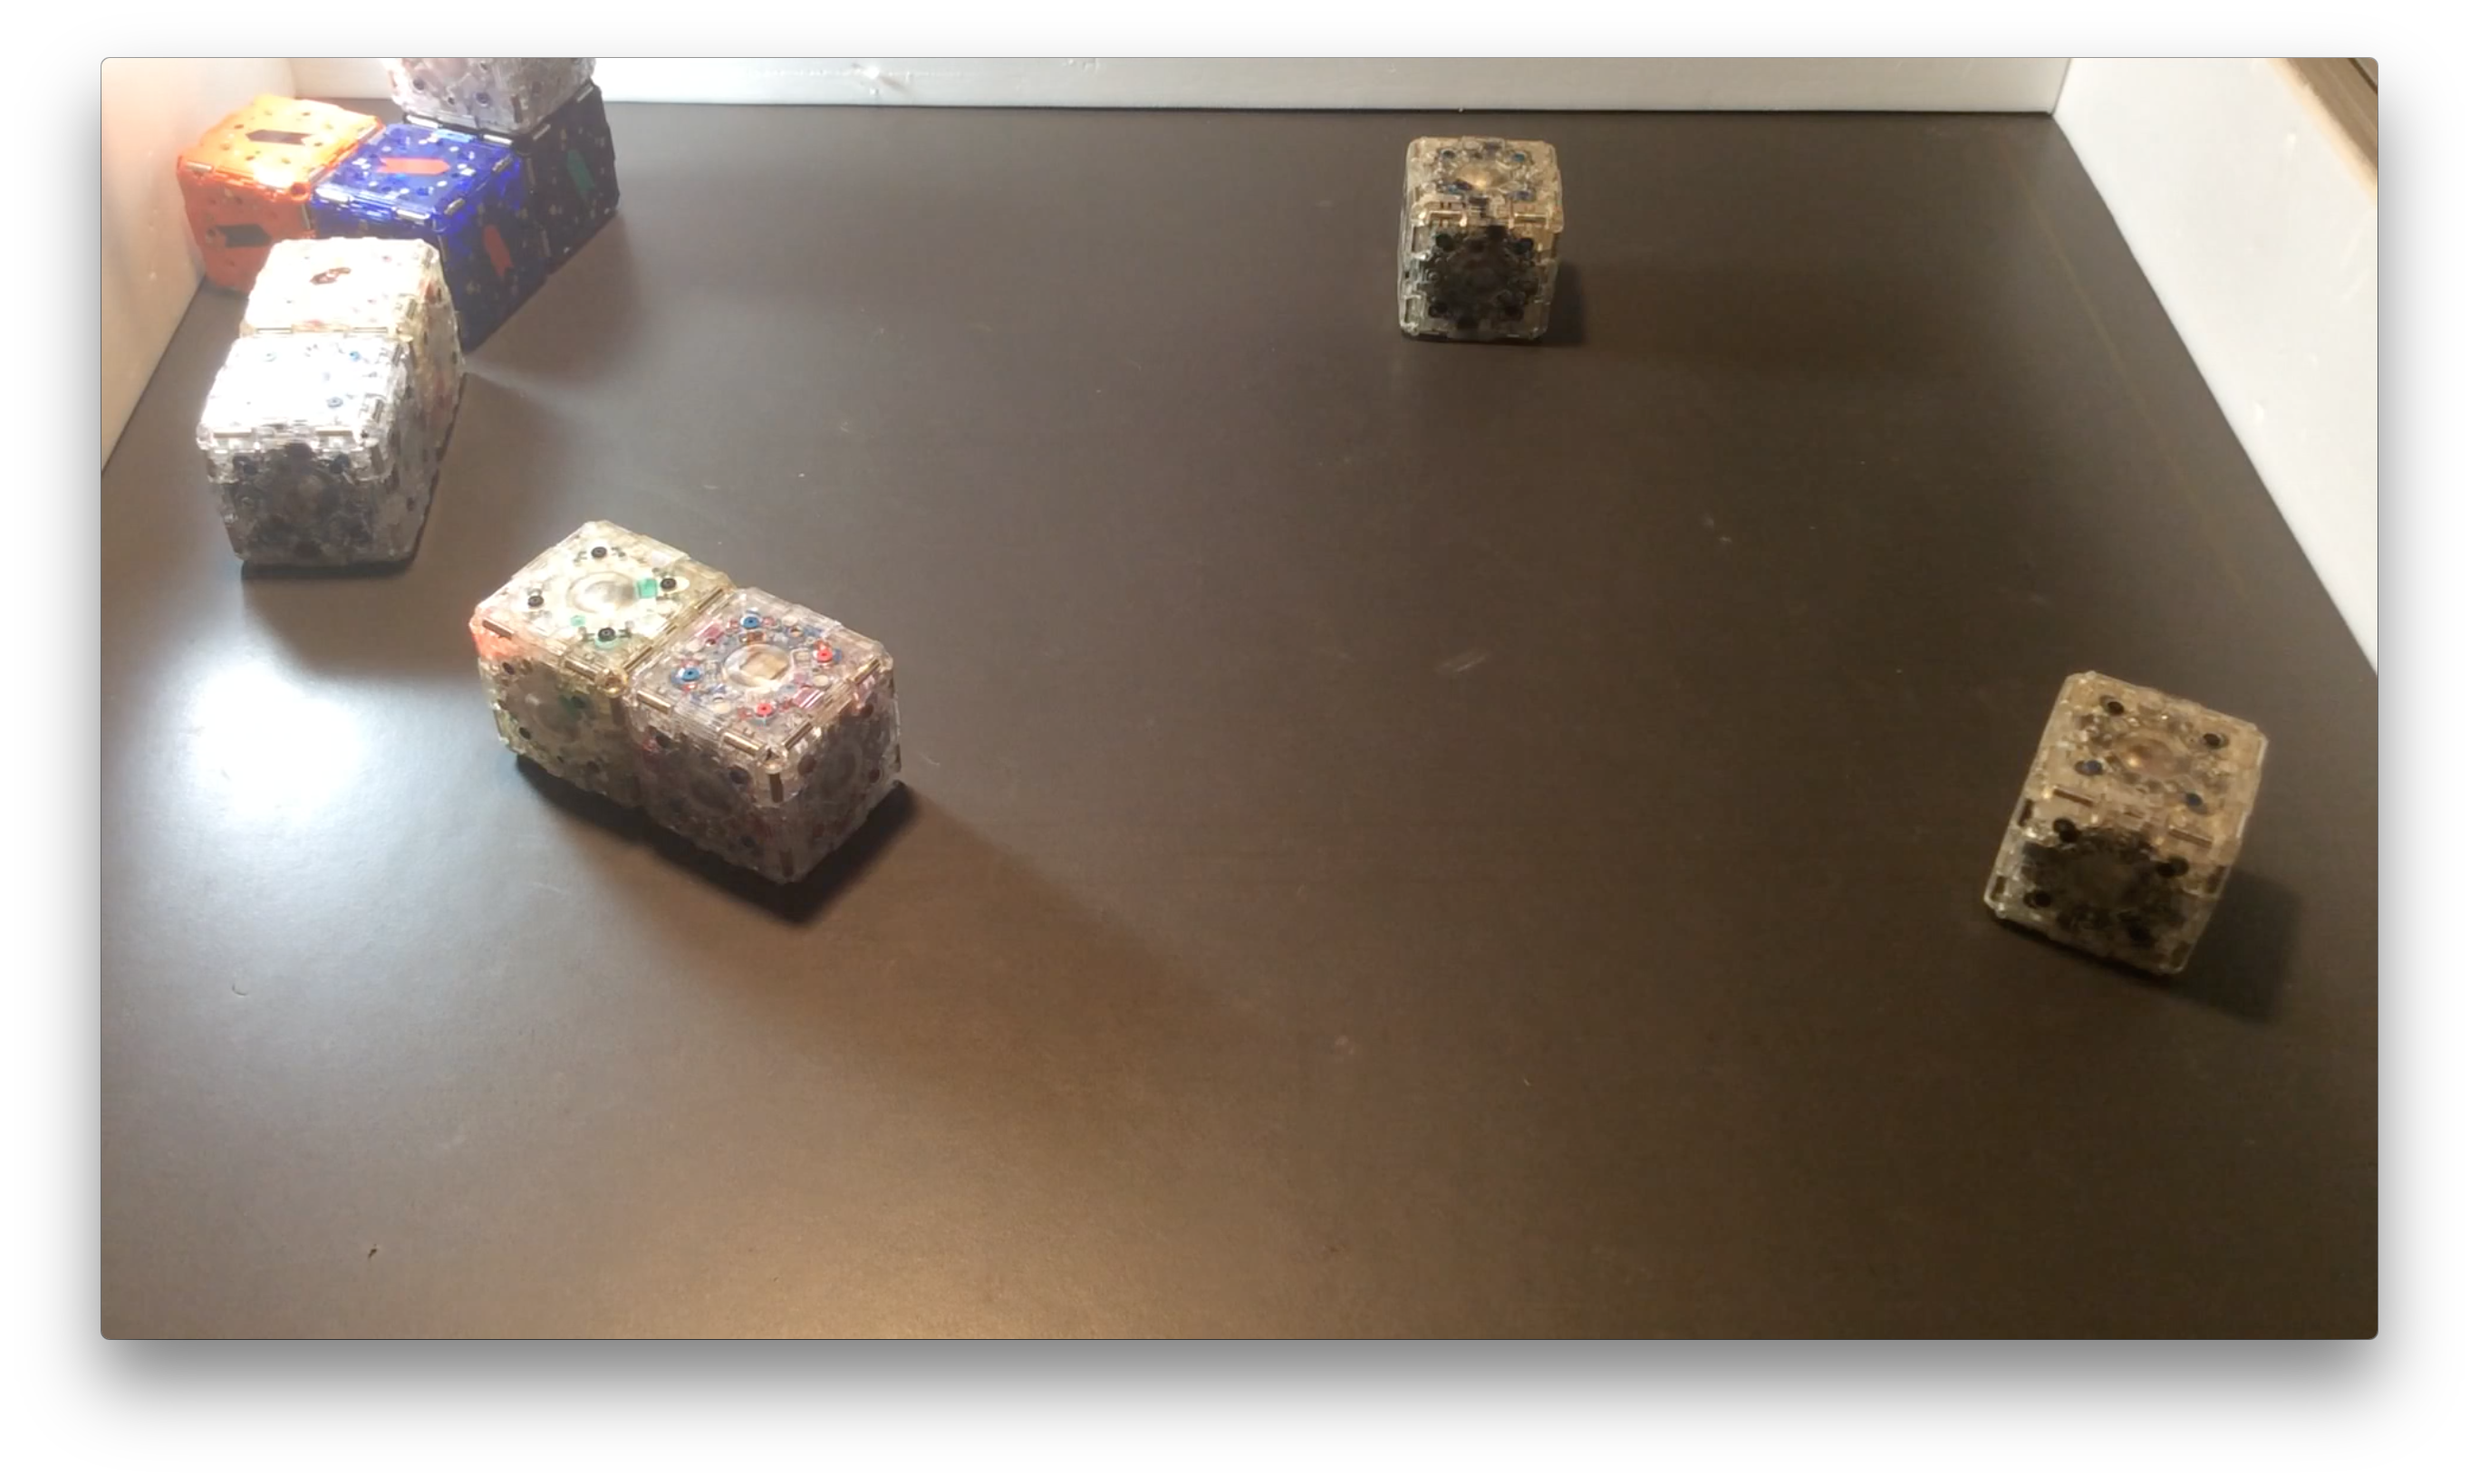
\includegraphics[width = \linewidth]{figures/4-320.png}};
		\node[opacity = 0.5, fill = white, rounded corners] at (-0.5,-0.5) {t = 320 s};
		\end{tikzpicture}
	\end{subfigure}
	\begin{subfigure}[b]{0.32\linewidth}
		\begin{tikzpicture}[]	
		\node[opacity = 0.95] at (0,0) {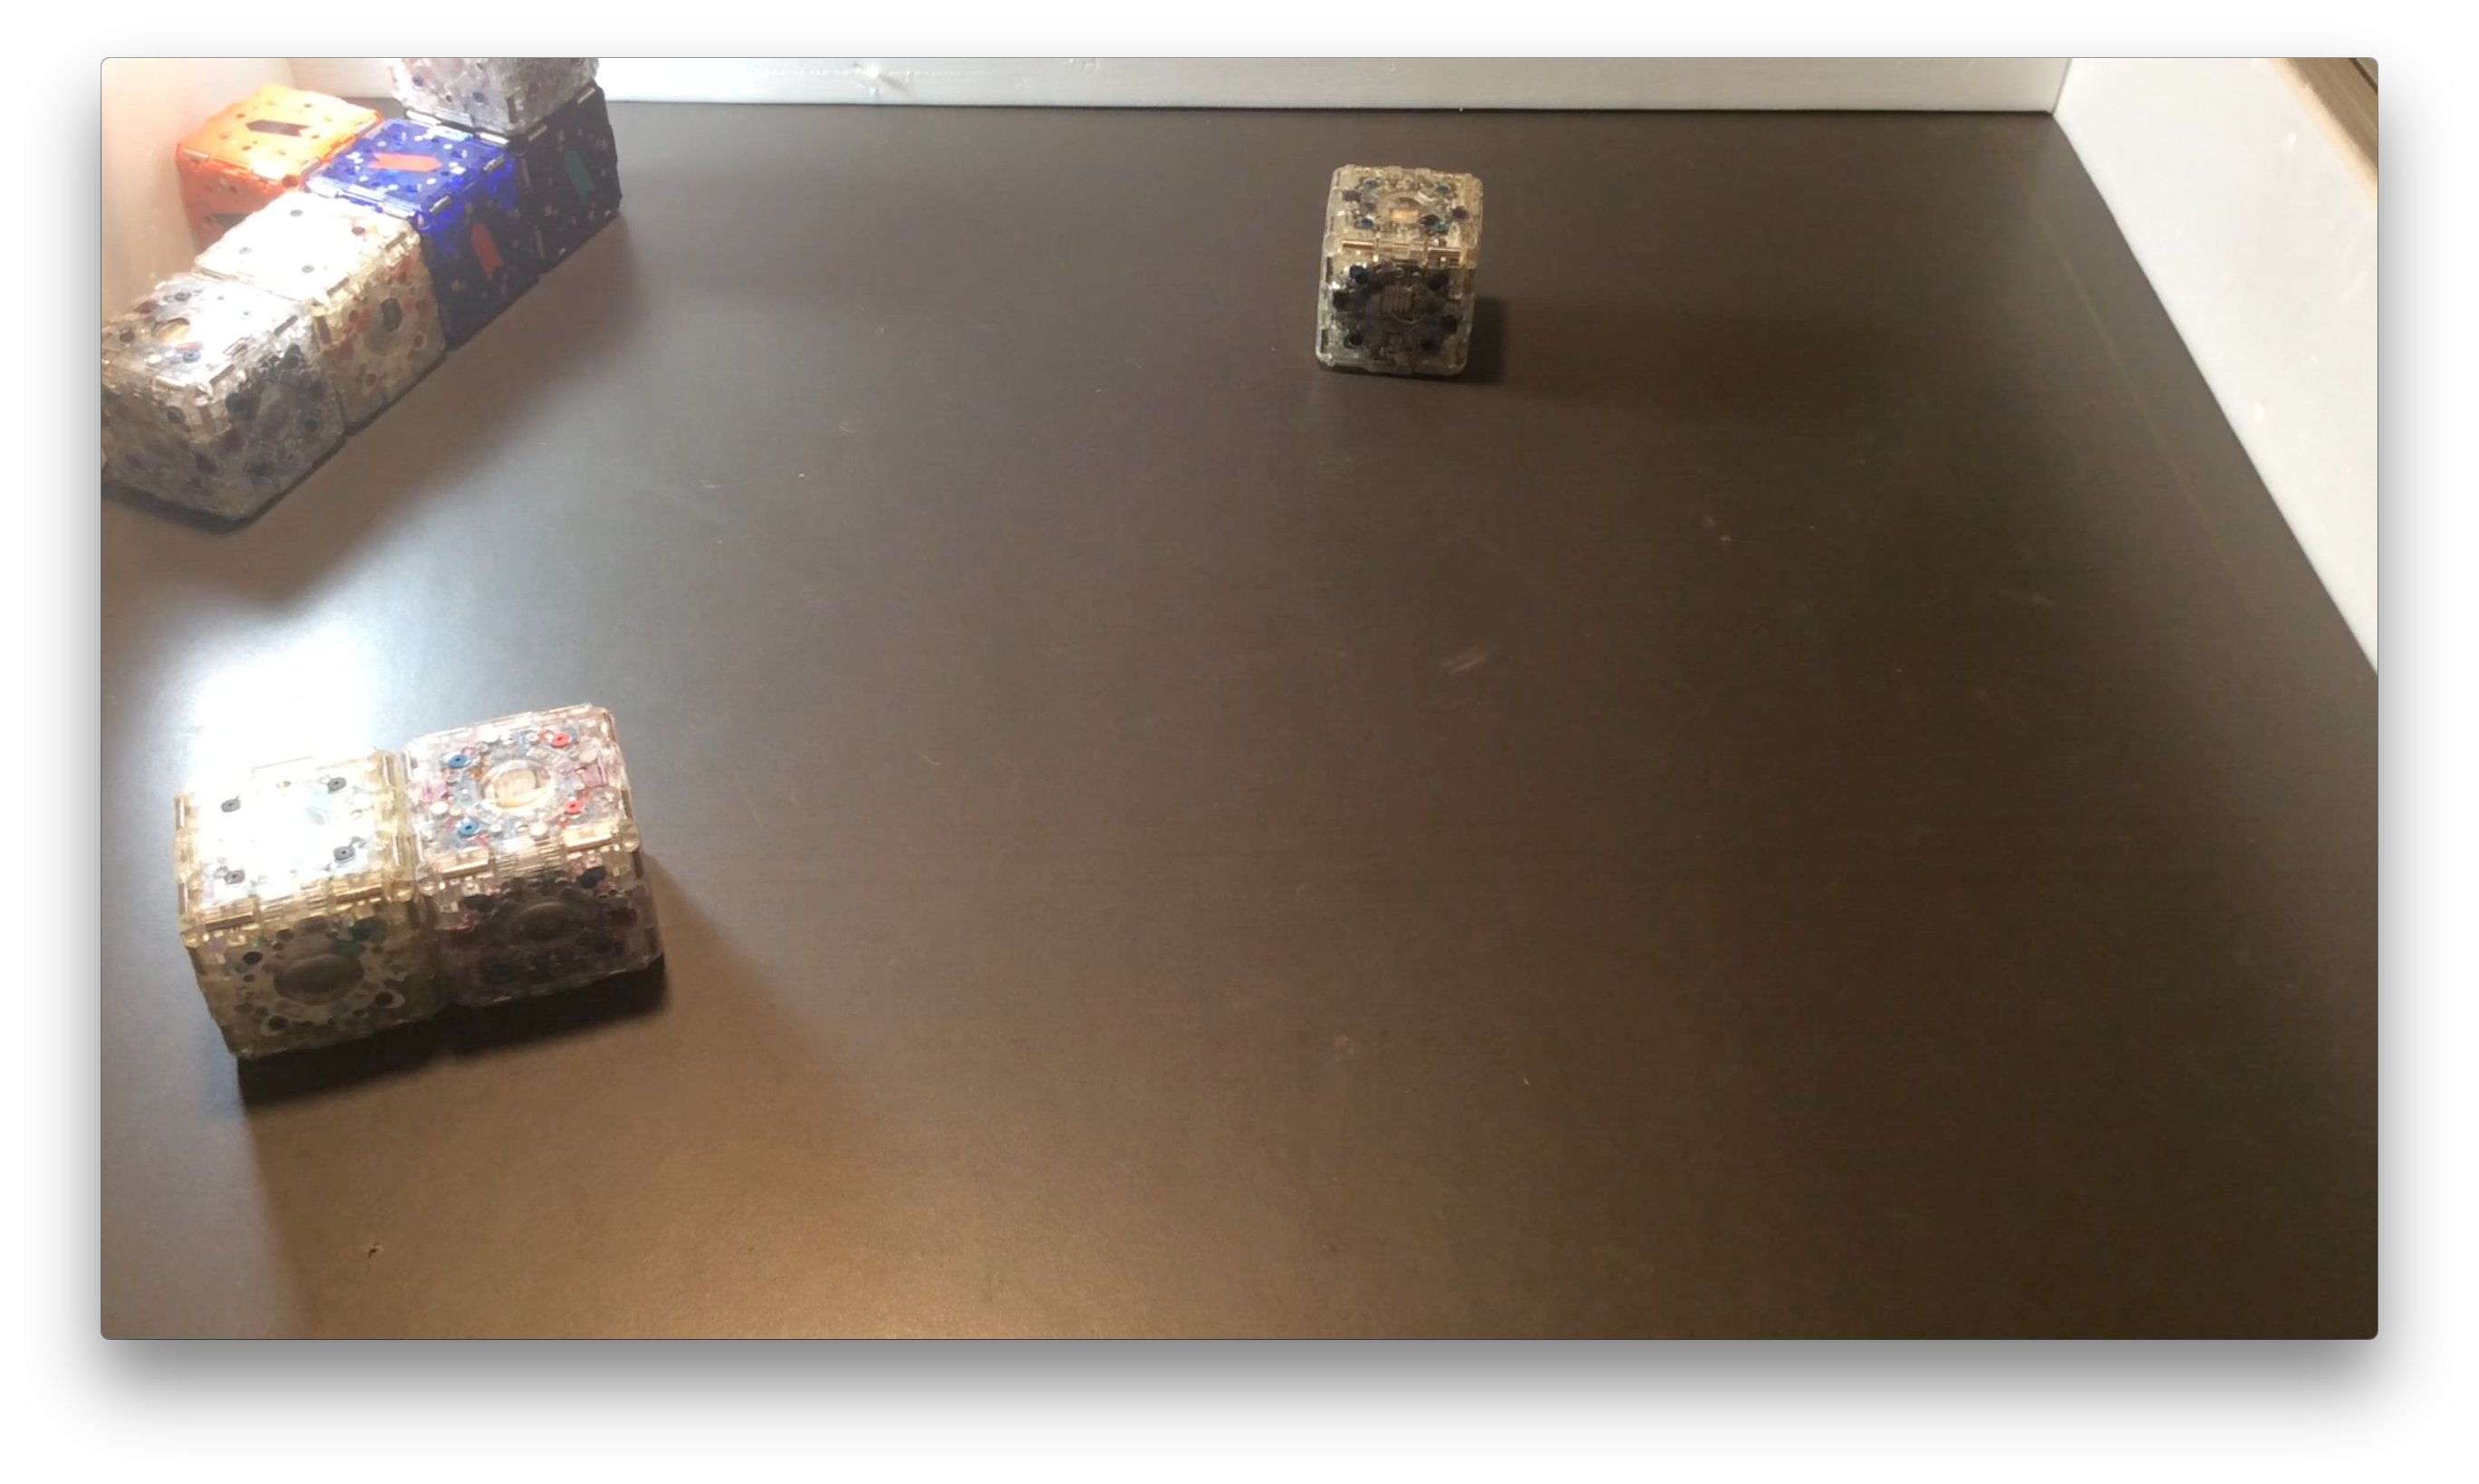
\includegraphics[width = \linewidth]{figures/5-500.png}};
		\node[opacity = 0.5, fill = white, rounded corners] at (-0.5,-0.5) {t = 500 s};
		\end{tikzpicture} 
	\end{subfigure}
	\begin{subfigure}[b]{0.32\linewidth}
		\begin{tikzpicture}[]	
		\node[opacity = 0.95] at (0,0) {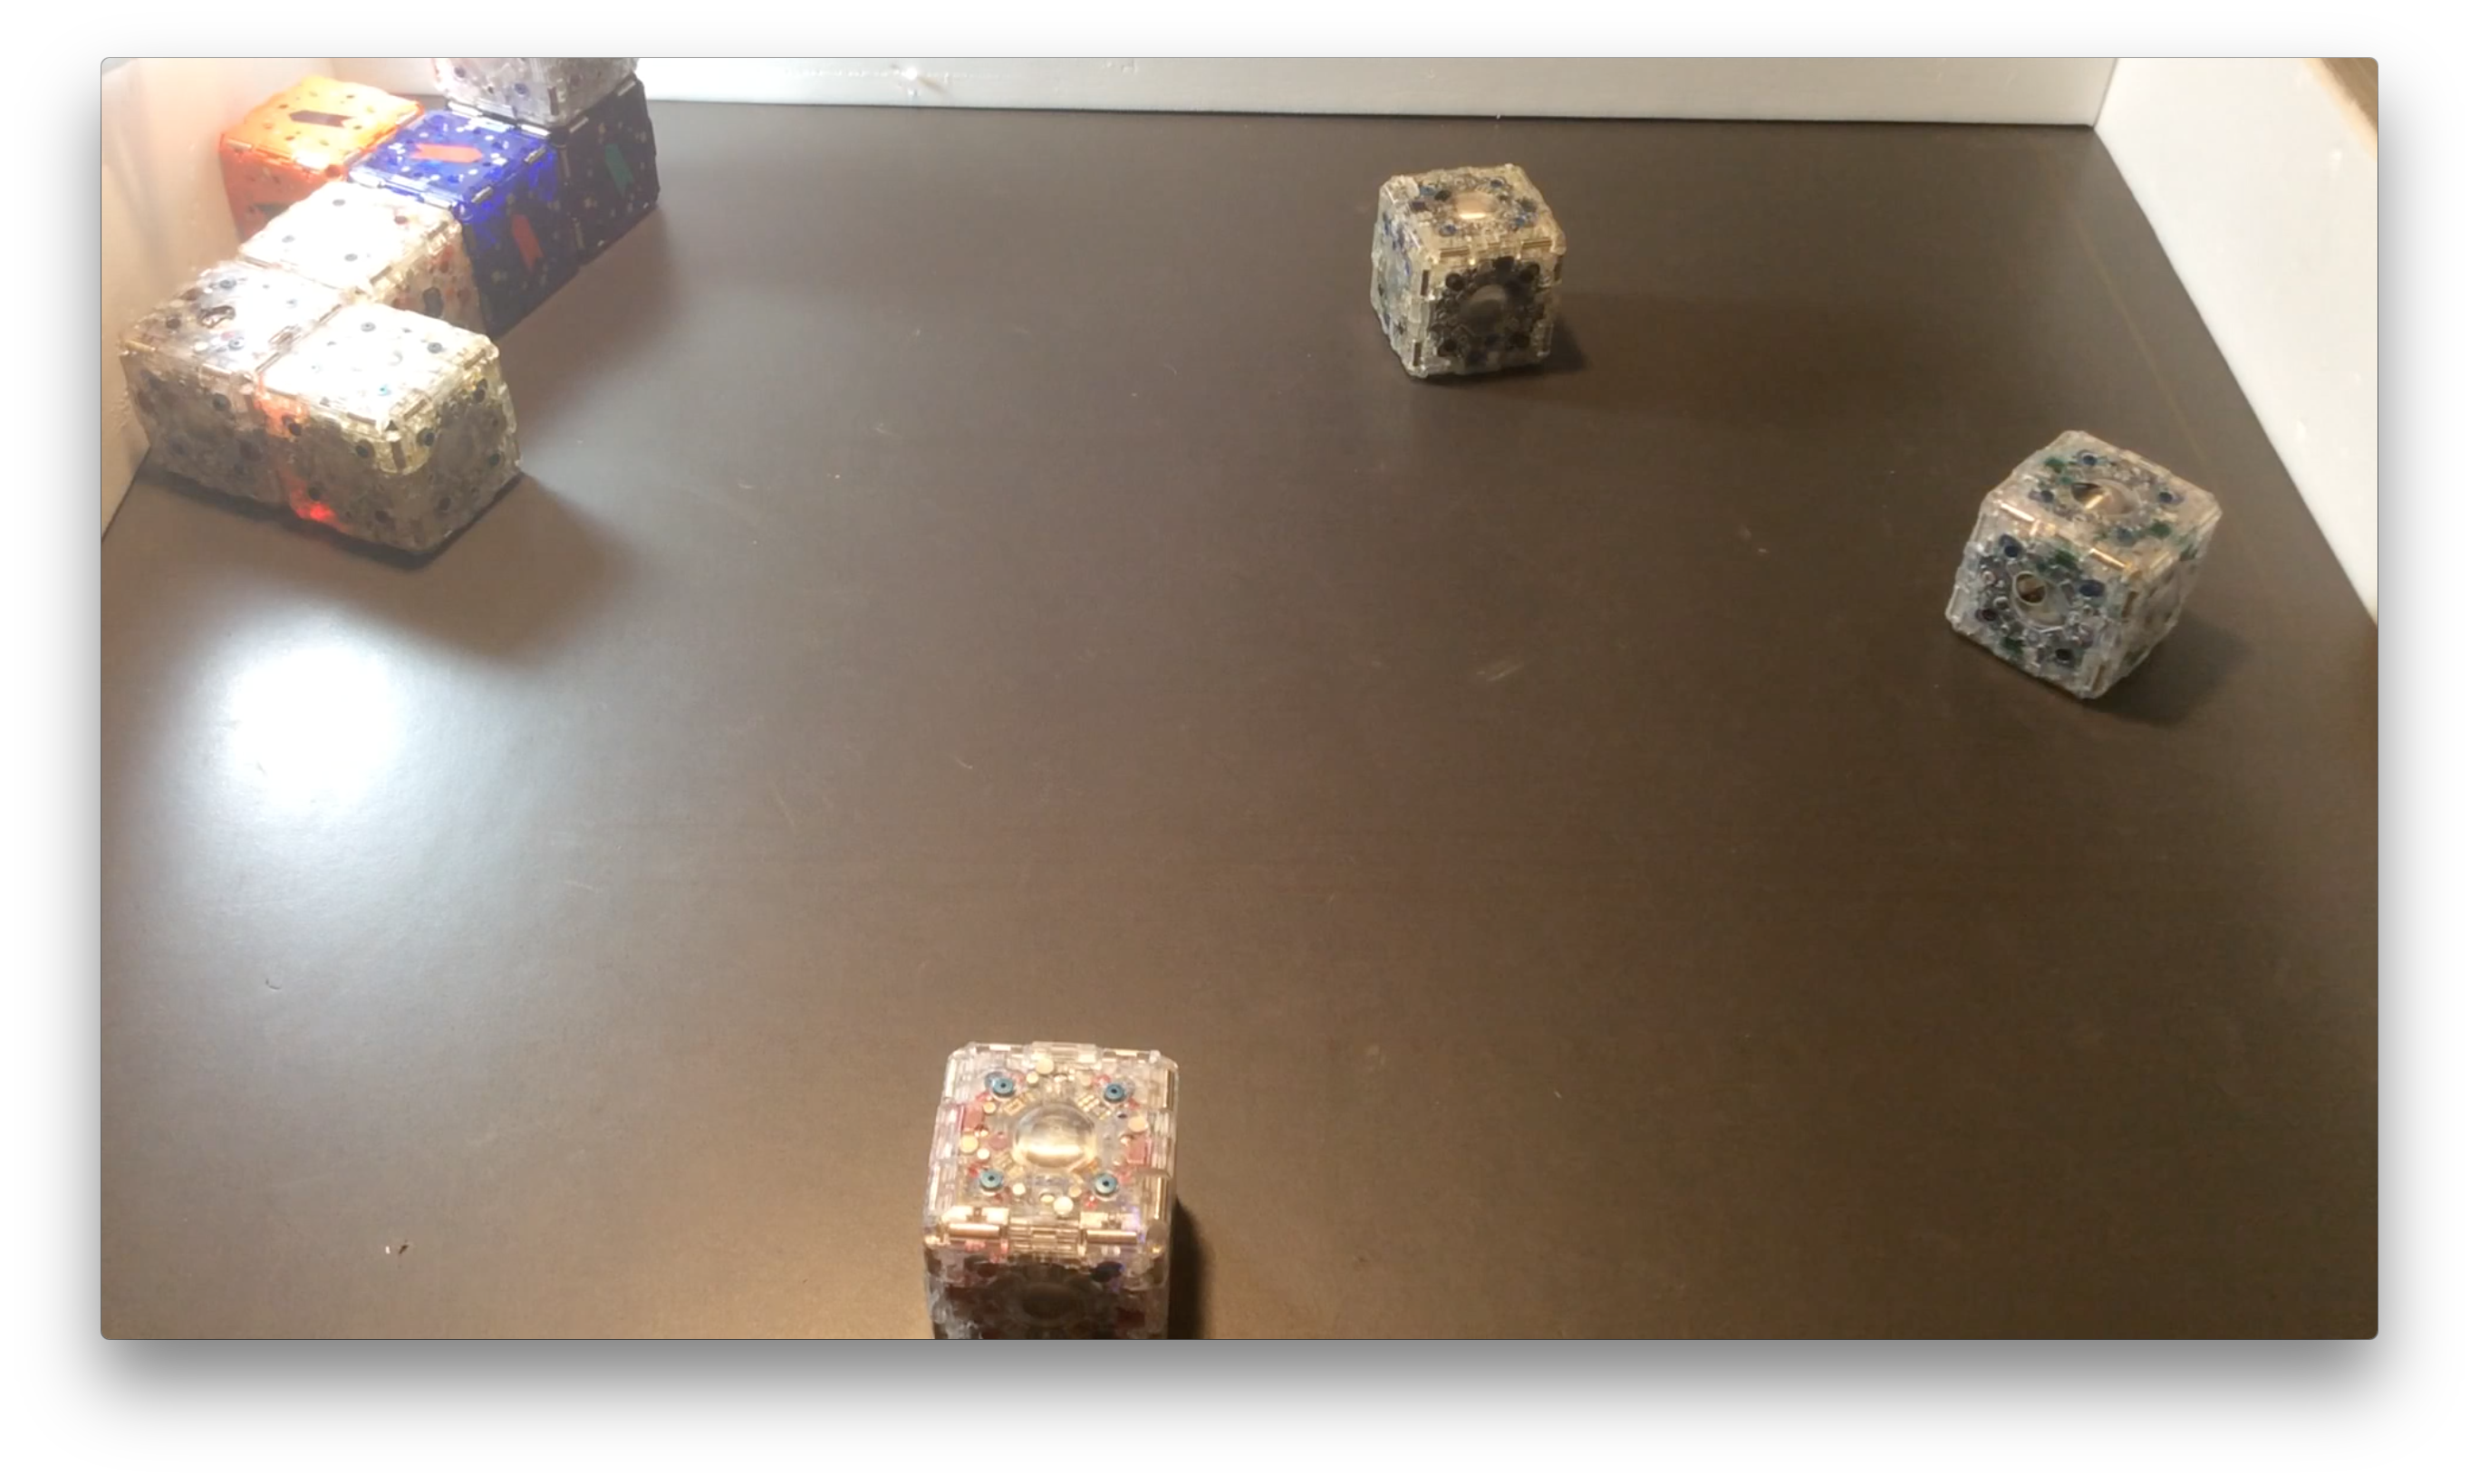
\includegraphics[width = \linewidth]{figures/6-600.png}};
		\node[opacity = 0.5, fill = white, rounded corners] at (-0.5,-0.5) {t = 600 s};
		\end{tikzpicture}
	\end{subfigure}
	
	\caption{This experiment illustrates the light guided aggregation behavior.}
	
	\label{fig:LightExperiment}
\end{figure}
